\documentclass[aspectratio=169,10pt]{beamer}

\usetheme{Madrid}
\usecolortheme{default}
\setbeamertemplate{navigation symbols}{}
\setbeamertemplate{footline}[frame number]

\usepackage{amsmath,amssymb,booktabs,mathtools}
\usepackage{hyperref}
\usepackage{graphicx}
\usepackage{tikz}
\usetikzlibrary{arrows.meta,positioning,decorations.pathreplacing,shapes.geometric}

% Semantic colors
\definecolor{positive}{HTML}{0173B2}
\definecolor{negative}{HTML}{DE8F05}
\definecolor{emphasis}{HTML}{029E73}
\definecolor{neutral}{gray}{0.55}
\definecolor{cbPurple}{HTML}{CC78BC}
\newcommand{\pos}[1]{\textcolor{positive}{#1}}
\newcommand{\con}[1]{\textcolor{negative}{#1}}
\newcommand{\HL}[1]{\textcolor{emphasis}{#1}}

\title{TWIST1\textsuperscript{+} FAP\textsuperscript{+} Fibroblasts in the Pathogenesis\\of Intestinal Fibrosis in Crohn's Disease}
\author{Presenter: [name]}
\institute{Shanghai Jiao Tong University}
\date{2026-03-10}

\begin{document}

% ============================================================
% SLIDE 1: Title
% ============================================================
\begin{frame}[plain]
\titlepage
\vfill
{\small Zhang Y, Wang J, Sun H, et al. \textit{J Clin Invest}. 2024;134(18):e179472.\\
Ruijin Hospital, Shanghai Jiao Tong University School of Medicine}
\end{frame}

% ============================================================
% SLIDE 2: Background — CD & Intestinal Fibrosis
% ============================================================
\begin{frame}{Background: Crohn's Disease \& Intestinal Fibrosis}
\begin{columns}[T]
\column{0.55\textwidth}
\begin{itemize}
  \item \textbf{Crohn's disease (CD)}: chronic gastrointestinal inflammatory disease
  \item \con{$\sim$50\% of CD patients} develop \textbf{intestinal fibrosis} $\rightarrow$ strictures
  \item Most patients require \textbf{surgical intervention}; 50\% relapse within 10 years
  \item \con{No FDA-approved antifibrotic therapy} for intestinal fibrosis
  \item Fibrosis = persistent abnormal activation of stromal cells $\rightarrow$ excessive \textbf{ECM} accumulation
\end{itemize}

\column{0.42\textwidth}
\begin{alertblock}{Key Gap}
The dominant \textbf{fibroblast subtype} responsible for excessive ECM deposition in intestinal fibrosis remains \con{unclear}.
\end{alertblock}
\vspace{6pt}
\begin{exampleblock}{This Study}
scRNA-seq on surgical samples from CD patients to identify key stromal cell subtype \& its activation mechanism.
\end{exampleblock}
\end{columns}
\end{frame}

% ============================================================
% SLIDE 3: Study Design
% ============================================================
\begin{frame}{Study Design \& Experimental Workflow}
\begin{center}
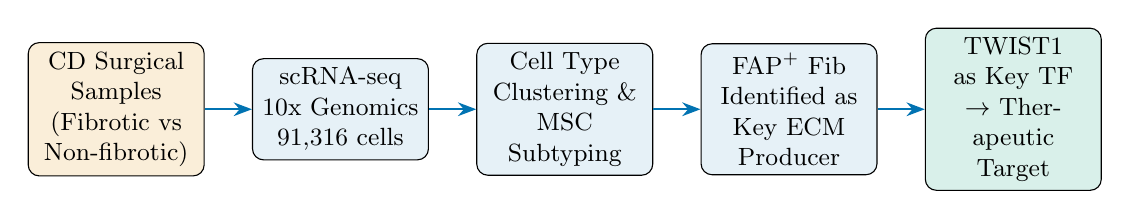
\begin{tikzpicture}[
  box/.style={draw, rounded corners=4pt, minimum width=2.0cm, minimum height=0.7cm,
              font=\small, fill=positive!10, text width=2.0cm, align=center},
  arr/.style={-{Stealth}, thick, positive},
  node distance=0.6cm
]
  \node[box, fill=negative!15] (sample) {CD Surgical\\Samples\\(Fibrotic vs\\Non-fibrotic)};
  \node[box, right=of sample] (scrna) {scRNA-seq\\10x Genomics\\91,316 cells};
  \node[box, right=of scrna] (cluster) {Cell Type\\Clustering \&\\MSC Subtyping};
  \node[box, right=of cluster] (fap) {FAP$^+$ Fib\\Identified as\\Key ECM\\Producer};
  \node[box, right=of fap, fill=emphasis!15] (twist) {TWIST1\\as Key TF\\$\rightarrow$ Therapeutic\\Target};

  \draw[arr] (sample) -- (scrna);
  \draw[arr] (scrna) -- (cluster);
  \draw[arr] (cluster) -- (fap);
  \draw[arr] (fap) -- (twist);
\end{tikzpicture}
\end{center}
\vspace{4pt}

\begin{columns}[T]
\column{0.48\textwidth}
\textbf{Validation approaches:}
\begin{itemize}
  \item Immunofluorescence (IF) \& Flow cytometry
  \item FACS + qPCR on sorted cells
  \item Multiplex IF (mIF)
\end{itemize}

\column{0.48\textwidth}
\textbf{Functional studies:}
\begin{itemize}
  \item DSS mouse colitis-fibrosis model
  \item Col1a2-CreERT2 Twist1$^{fl/fl}$ conditional KO
  \item Harmine (TWIST1 inhibitor) treatment
\end{itemize}
\end{columns}
\end{frame}

% ============================================================
% SLIDE 4: Cellular Landscape (Fig 1)
% ============================================================
\begin{frame}{Cellular Landscape of Fibrotic Intestine (Fig.\,1)}
\begin{columns}[T]
\column{0.55\textwidth}
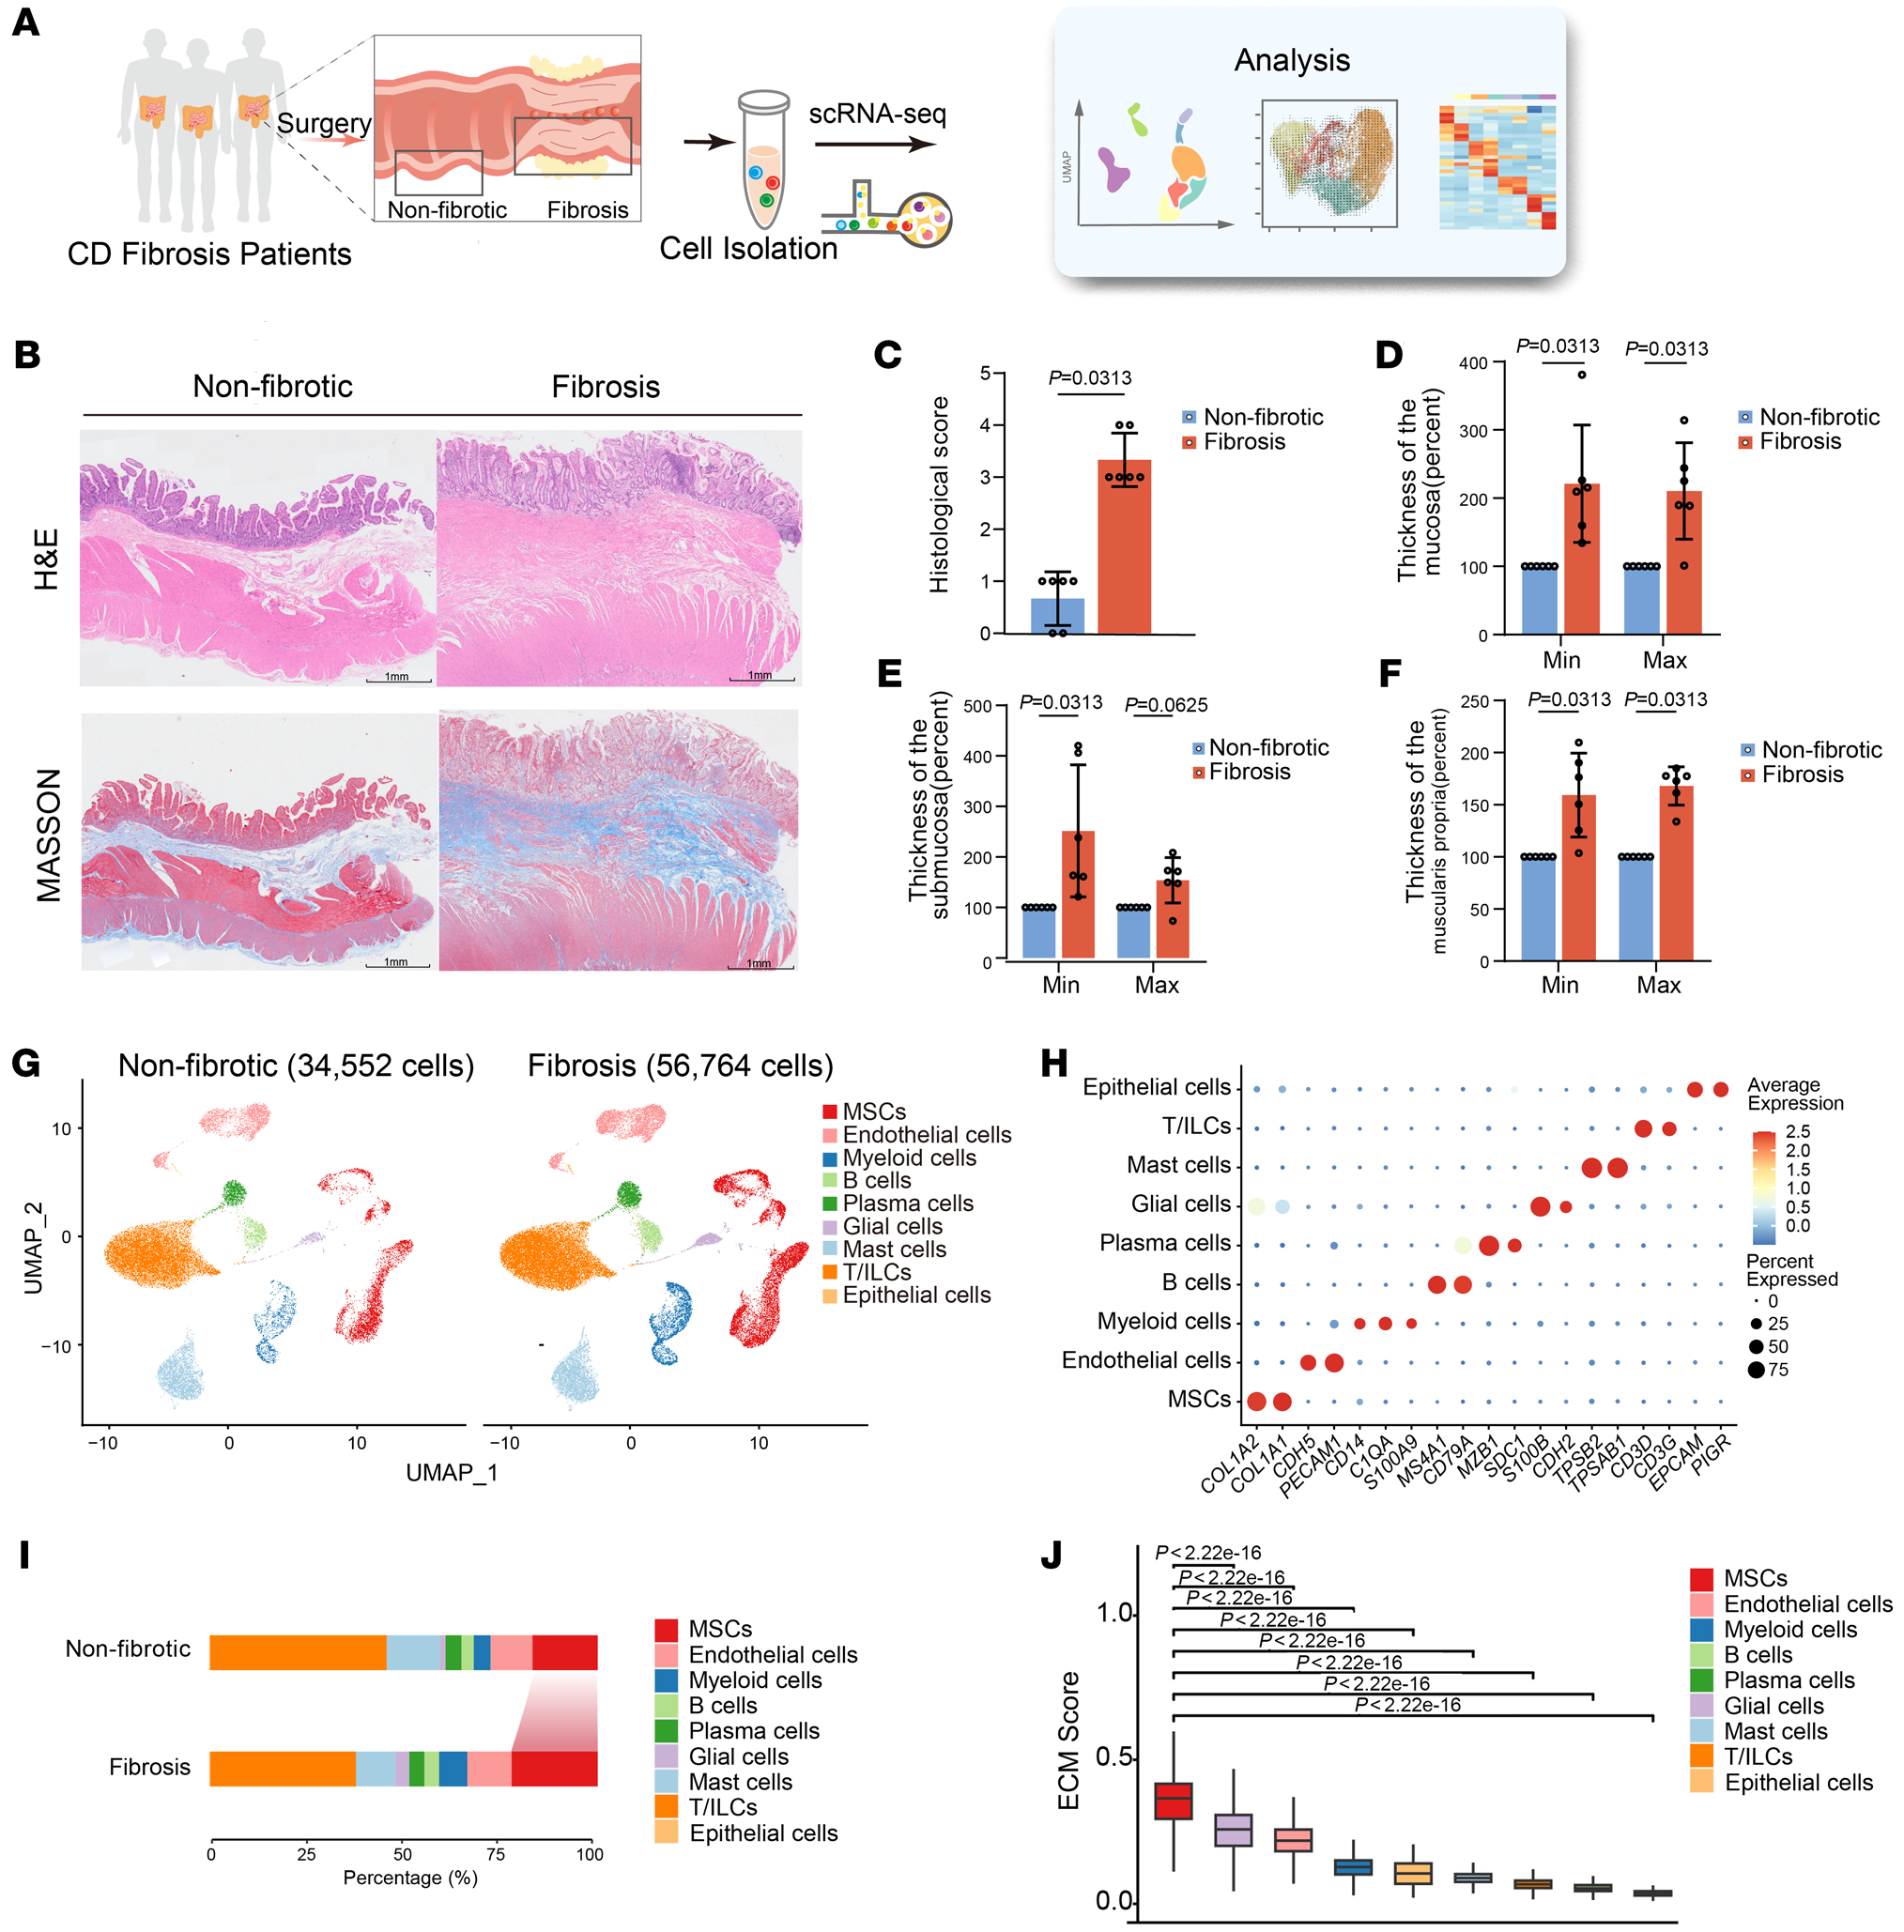
\includegraphics[width=\textwidth, trim=0 550 0 0, clip]{figures/fig1-img0.png}
{\tiny Source: Zhang et al., JCI 2024, Fig.\,1}

\column{0.42\textwidth}
\textbf{Sample}: 6 fibrotic + 6 non-fibrotic ileal tissues
\vspace{4pt}

\textbf{Results}:
\begin{itemize}
  \item \textbf{91,316 cells} after QC $\rightarrow$ \textbf{9 major cell types}
  \item MSC \& myeloid cells: \pos{increased} in fibrotic tissue
  \item T/ILCs \& mast cells: \con{decreased}
\end{itemize}
\vspace{4pt}

\begin{alertblock}{Key Finding}
\textbf{MSCs} exhibited the \HL{highest ECM score} in fibrotic areas $\rightarrow$ pivotal role in ECM production.
\end{alertblock}
\end{columns}
\end{frame}

% ============================================================
% SLIDE 5: MSC Heterogeneity (Fig 2)
% ============================================================
\begin{frame}{MSC Heterogeneity: FAP$^+$ Fibroblasts Enriched in Fibrosis (Fig.\,2)}
\begin{columns}[T]
\column{0.55\textwidth}
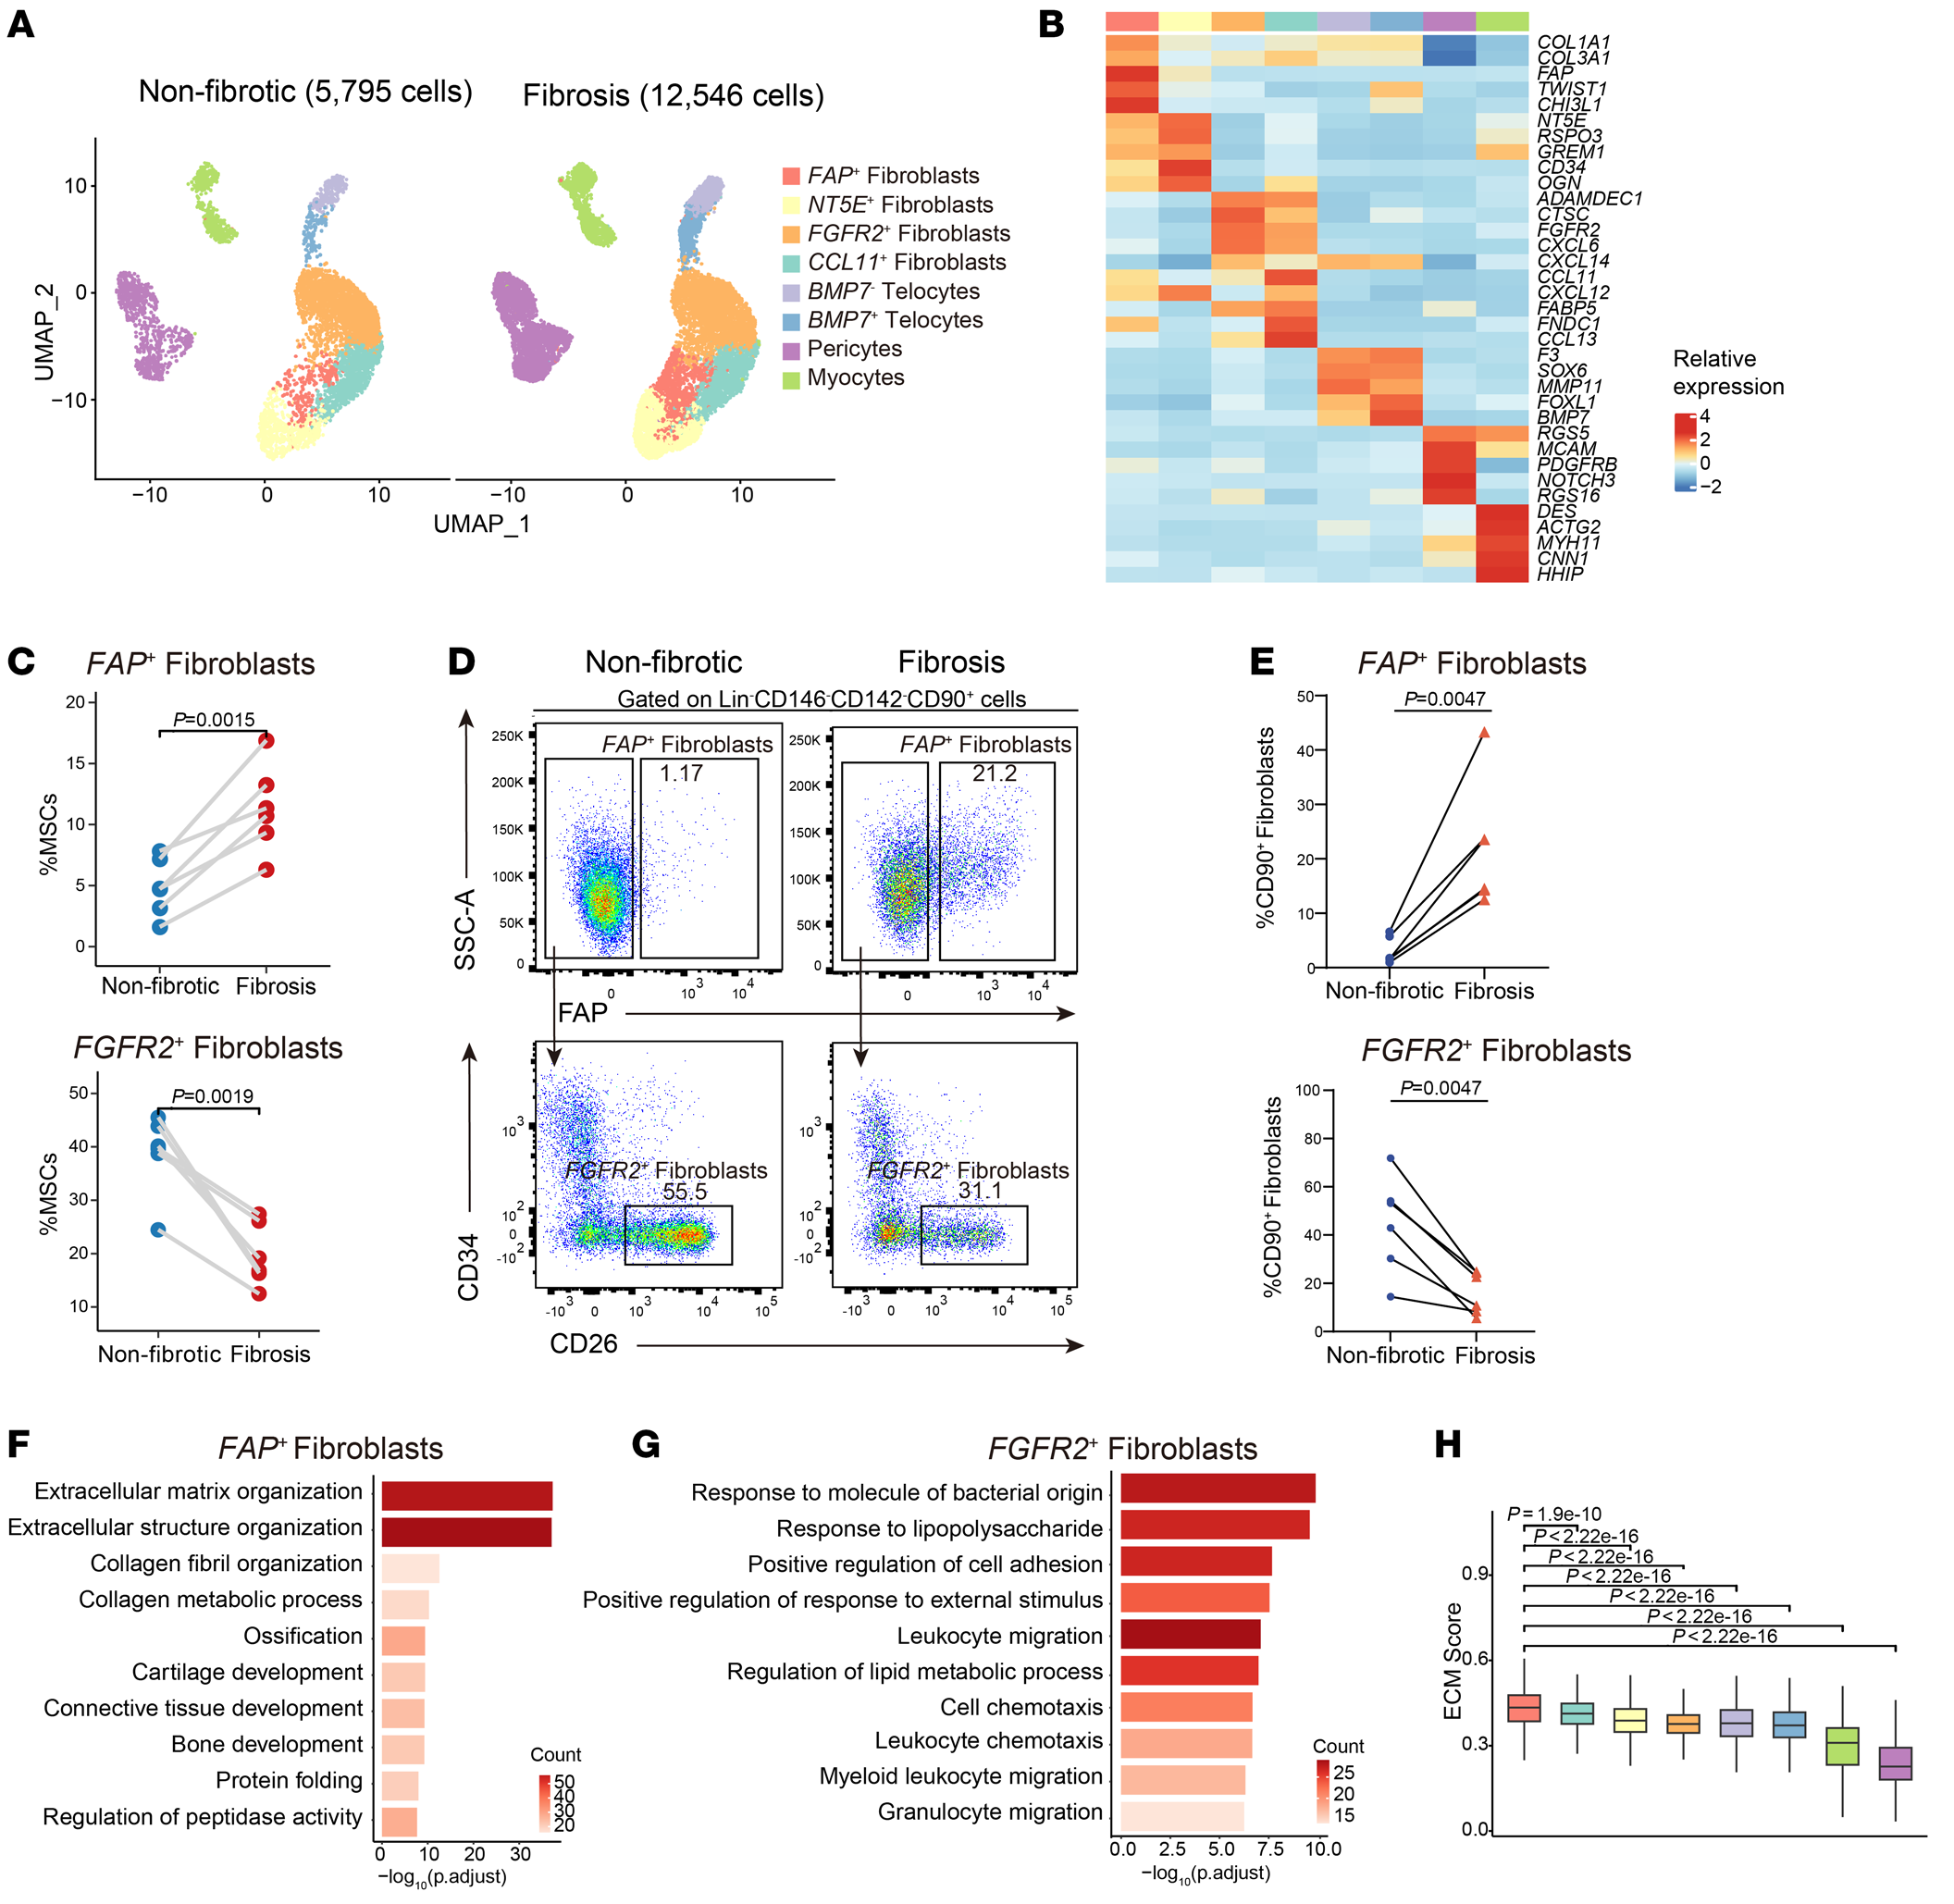
\includegraphics[width=\textwidth, trim=0 500 0 0, clip]{figures/fig2-img0.png}
{\tiny Source: Zhang et al., JCI 2024, Fig.\,2}

\column{0.42\textwidth}
\textbf{MSC subclustering} $\rightarrow$ 4 major subsets:
\begin{itemize}
  \item Fibroblasts, Telocytes, Pericytes, Myocytes
\end{itemize}
\vspace{4pt}

\textbf{4 fibroblast subtypes}:
\begin{itemize}
  \item NT5E$^+$, \pos{FAP$^+$}, CCL11$^+$, FGFR2$^+$
\end{itemize}
\vspace{4pt}

\textbf{Key observations}:
\begin{itemize}
  \item \pos{FAP$^+$} fibroblasts: \HL{significantly enriched} in fibrotic areas ($P = 0.0015$)
  \item FGFR2$^+$ fibroblasts: more abundant in non-fibrotic areas
  \item FAP$^+$ fibroblasts: \HL{highest ECM score} among all MSC subsets
  \item GO enrichment: ECM \& structural organization
\end{itemize}
\end{columns}
\end{frame}

% ============================================================
% SLIDE 6: FAP+ Fibroblasts Validation (Fig 3A-C)
% ============================================================
\begin{frame}{FAP$^+$ Fibroblasts: Key ECM Producers in Fibrosis (Fig.\,3)}
\begin{columns}[T]
\column{0.52\textwidth}
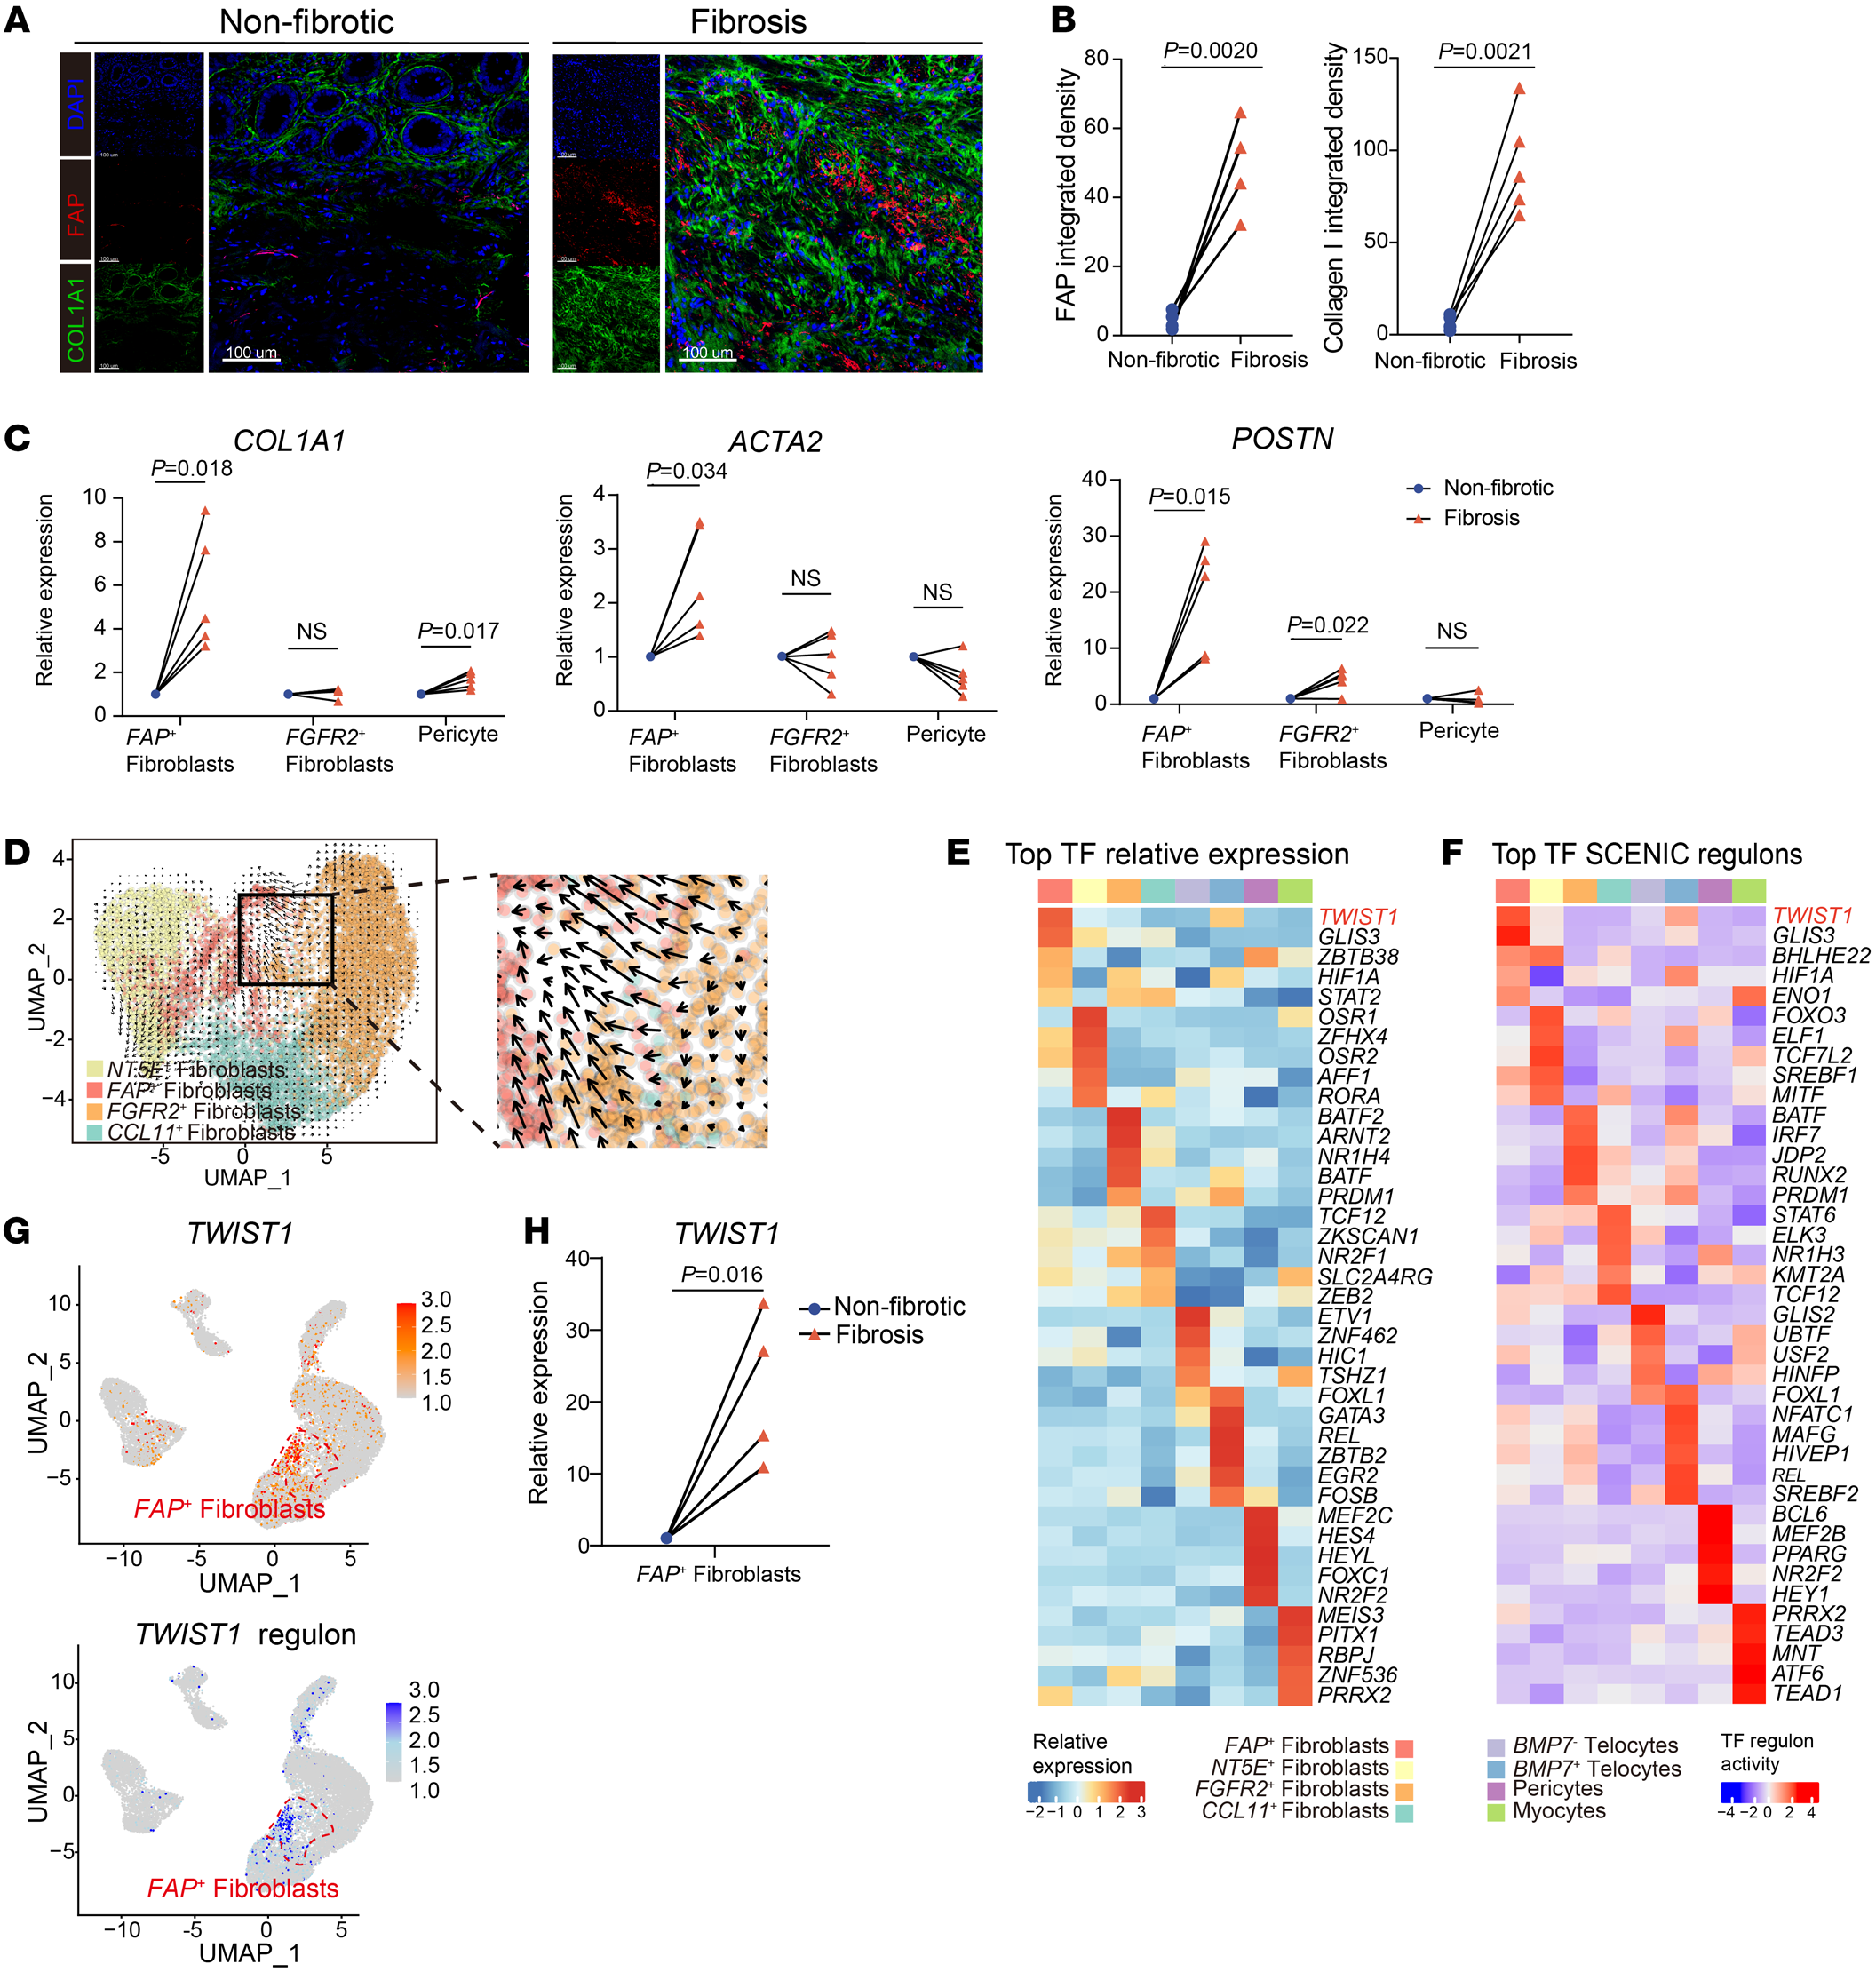
\includegraphics[width=\textwidth, trim=0 1200 1000 0, clip]{figures/fig3-img0.png}
{\tiny Source: Zhang et al., JCI 2024, Fig.\,3A--C}

\column{0.45\textwidth}
\textbf{IF validation}:
\begin{itemize}
  \item FAP$^+$ fibroblasts \HL{co-localized with COL1A1} in fibrotic areas
  \item Absent in non-fibrotic intestinal samples
\end{itemize}
\vspace{4pt}

\textbf{FACS + qPCR on sorted FAP$^+$ fibroblasts}:
\begin{itemize}
  \item \textbf{COL1A1} $\uparrow$ ($P = 0.018$)
  \item \textbf{ACTA2} ($\alpha$-SMA) $\uparrow$ ($P = 0.034$)
  \item \textbf{POSTN} $\uparrow$ ($P = 0.015$)
\end{itemize}
\vspace{4pt}

\begin{exampleblock}{Pseudotime Analysis}
RNA velocity \& Monocle: FAP$^+$ fibroblasts \textbf{differentiated from FGFR2$^+$} fibroblasts.
\end{exampleblock}
\end{columns}
\end{frame}

% ============================================================
% SLIDE 7: TWIST1 as Key TF (Fig 3D-H)
% ============================================================
\begin{frame}{TWIST1: Critical Transcription Factor for FAP$^+$ Differentiation (Fig.\,3)}
\begin{columns}[T]
\column{0.52\textwidth}
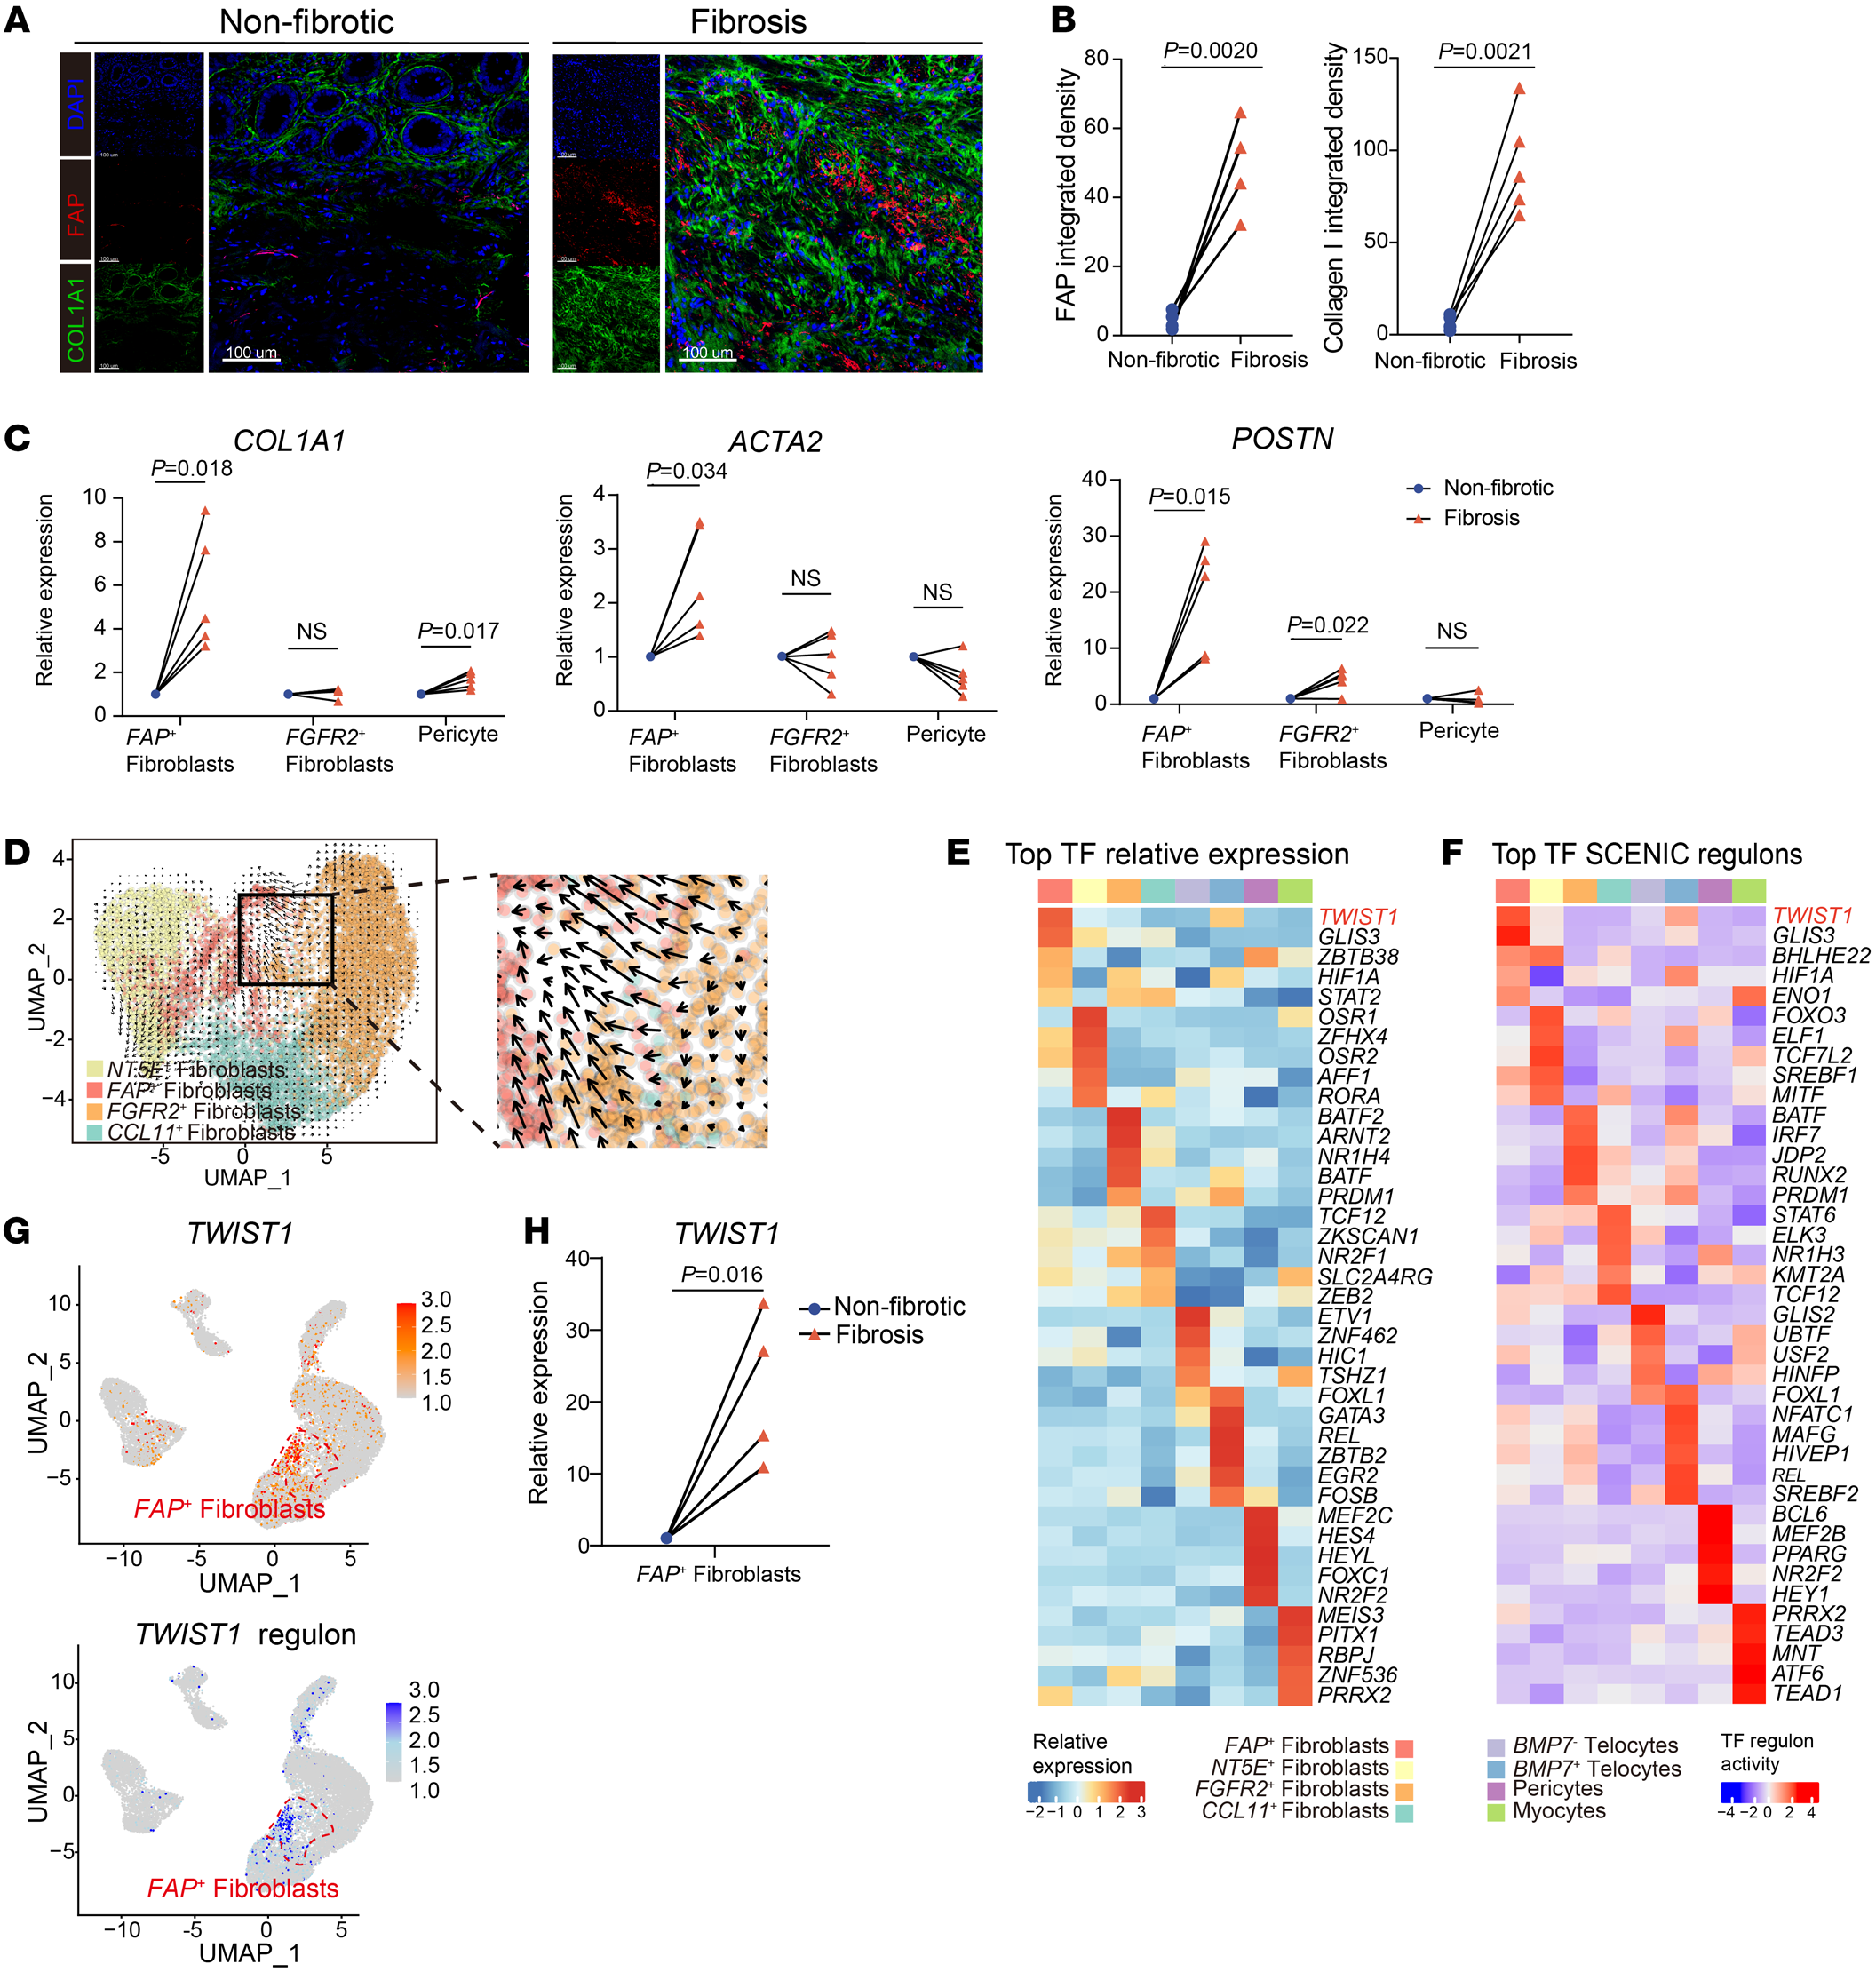
\includegraphics[width=\textwidth, trim=1000 0 0 1100, clip]{figures/fig3-img0.png}
{\tiny Source: Zhang et al., JCI 2024, Fig.\,3D--H}

\column{0.45\textwidth}
\textbf{SCENIC analysis}:
\begin{itemize}
  \item TWIST1 exhibited \HL{highest expression \& regulatory activity} in FAP$^+$ fibroblasts
\end{itemize}
\vspace{4pt}

\textbf{RNA velocity}:
\begin{itemize}
  \item Differentiation trajectory:\\FGFR2$^+$ $\rightarrow$ FAP$^+$ fibroblasts
  \item Fibrosis-related genes \textbf{upregulated} upon differentiation
\end{itemize}
\vspace{4pt}

\textbf{qPCR validation}:
\begin{itemize}
  \item TWIST1 mRNA \pos{upregulated} in fibrotic tissues
  \item TWIST1 mRNA \pos{upregulated} in FAP$^+$ fibroblasts from fibrotic sites
\end{itemize}
\vspace{4pt}

$\Rightarrow$ \textbf{TWIST1} = key TF driving FGFR2$^+$ $\rightarrow$ FAP$^+$ transition
\end{columns}
\end{frame}

% ============================================================
% SLIDE 8: Profibrotic Macrophages (Fig 4)
% ============================================================
\begin{frame}{Profibrotic CXCL9$^+$ Macrophages in Fibrotic Intestine (Fig.\,4)}
\begin{columns}[T]
\column{0.52\textwidth}
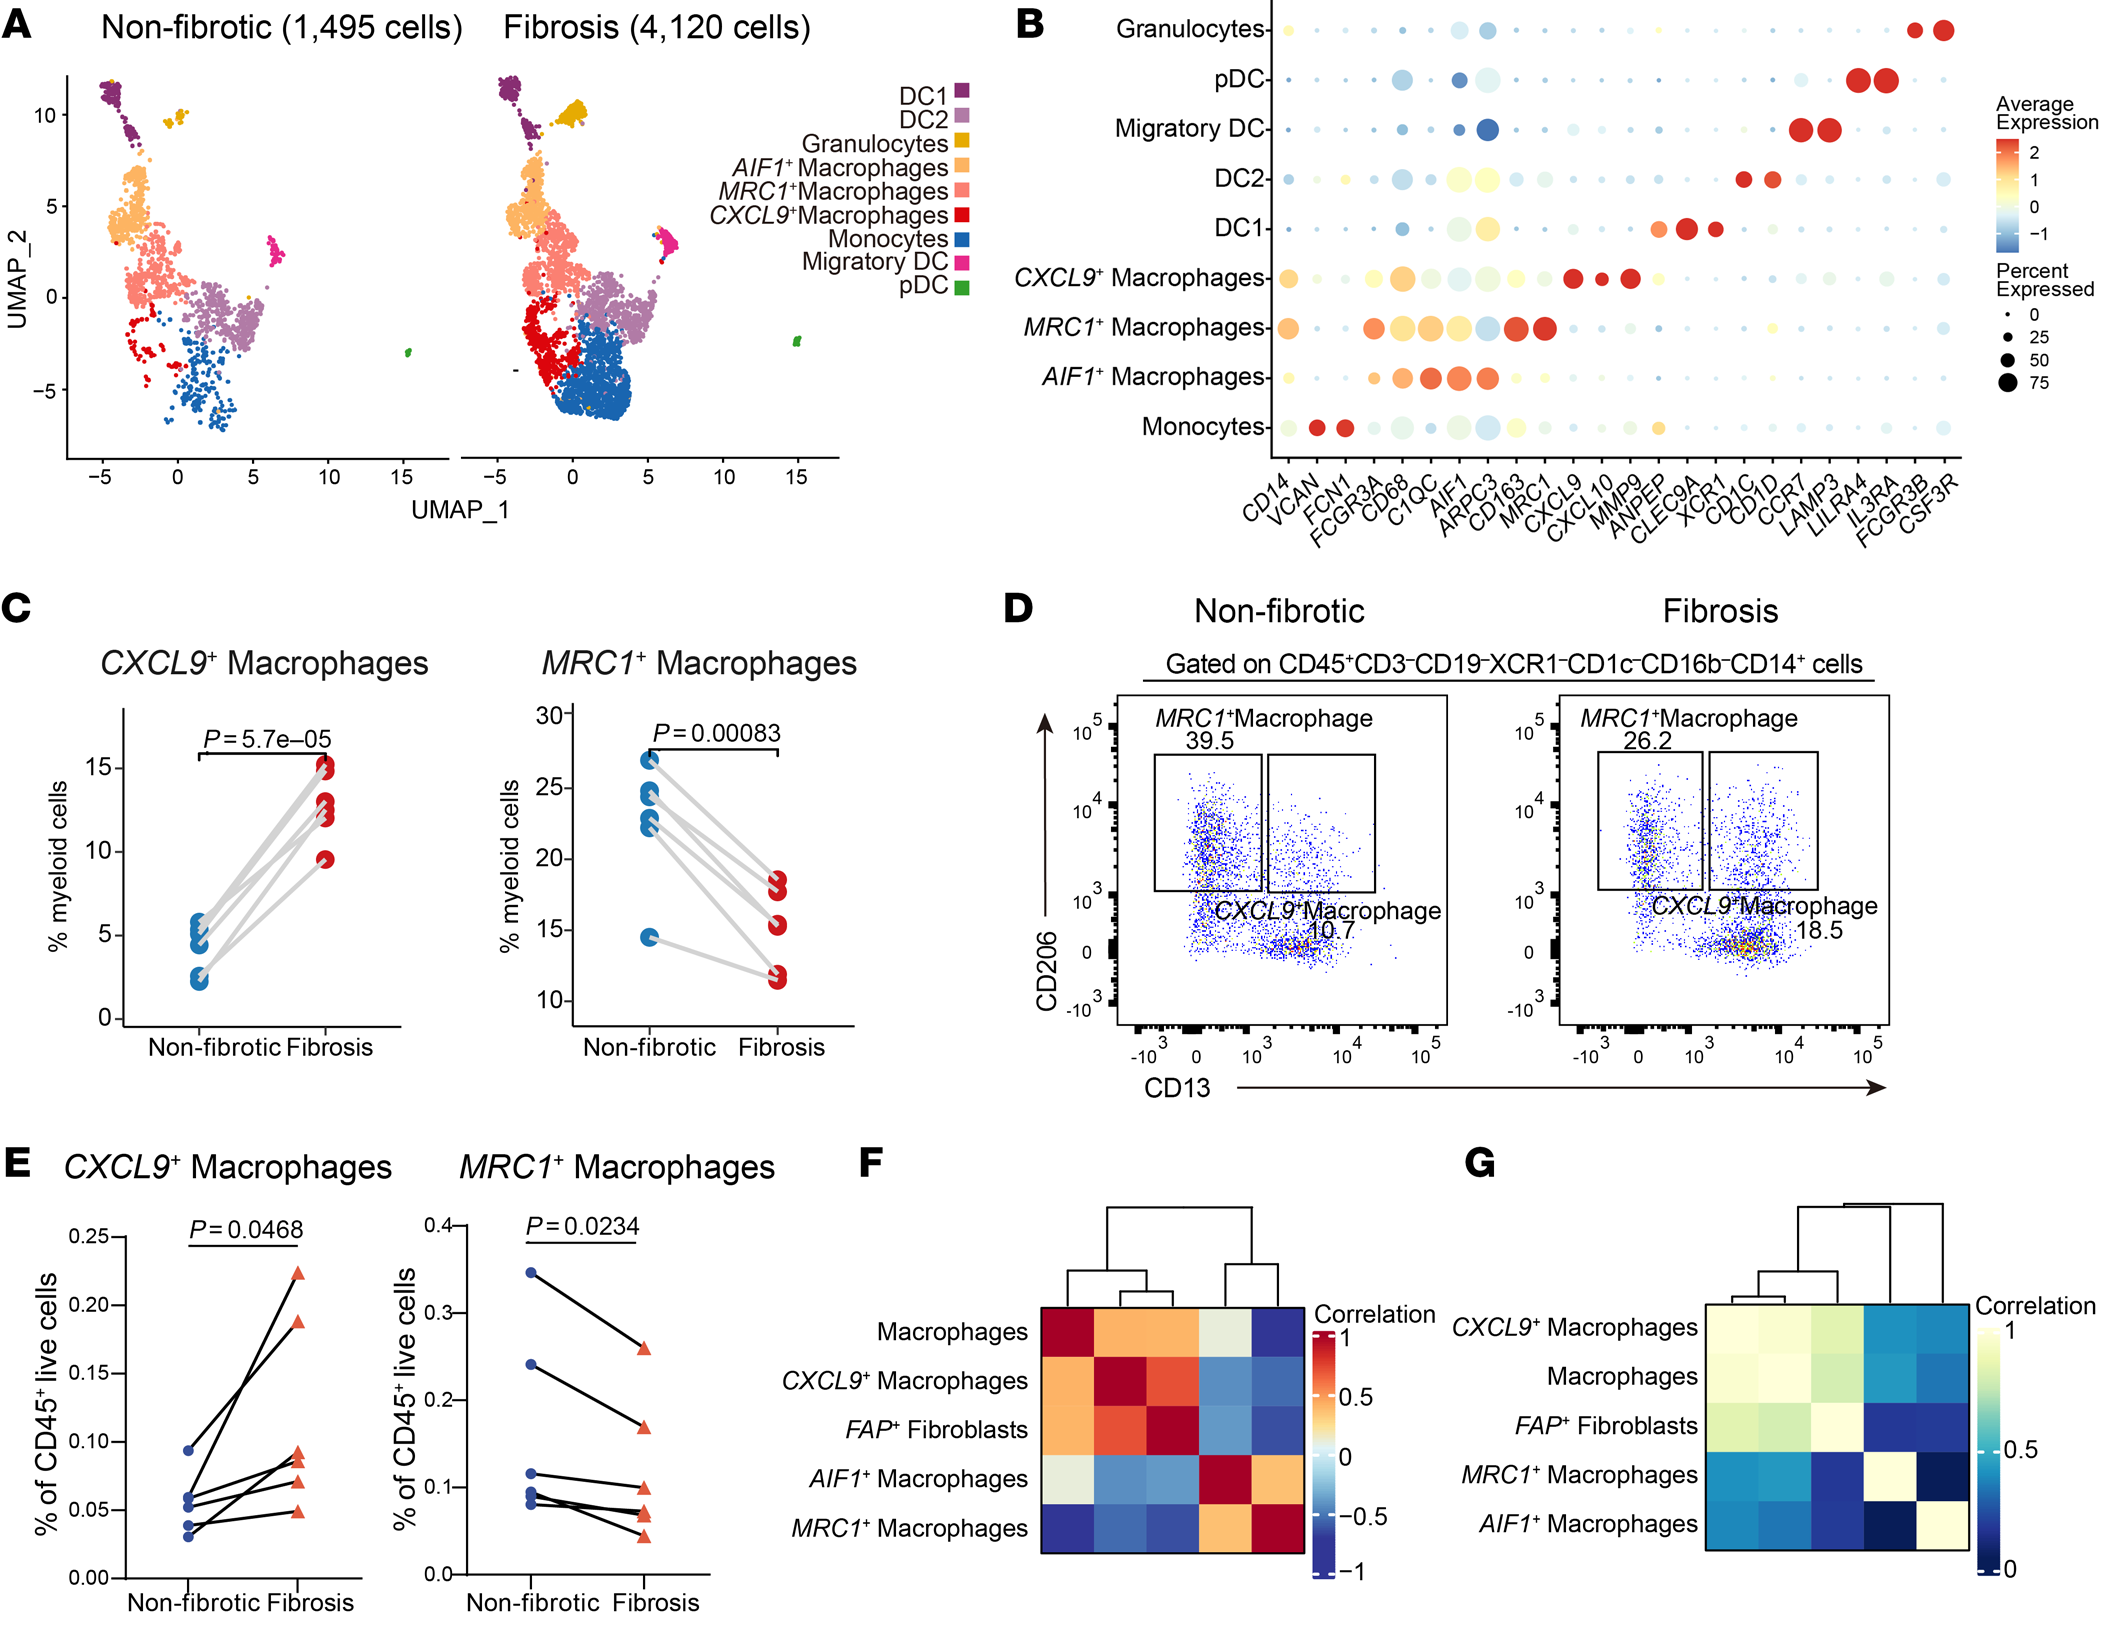
\includegraphics[width=\textwidth]{figures/fig4-img0.png}
{\tiny Source: Zhang et al., JCI 2024, Fig.\,4}

\column{0.45\textwidth}
\textbf{Myeloid subclustering}: 9 clusters, 3 macrophage subsets:
\begin{itemize}
  \item \pos{CXCL9$^+$}, MRC1$^+$, AIF1$^+$ macrophages
\end{itemize}
\vspace{4pt}

\textbf{Key findings}:
\begin{itemize}
  \item \pos{CXCL9$^+$ Mac}: \HL{enriched in fibrotic areas} ($P = 5.7 \times 10^{-5}$)
  \item MRC1$^+$ \& AIF1$^+$ Mac: decreased in fibrosis
  \item CXCL9$^+$ Mac: \con{highest profibrotic score}
  \item MRC1$^+$ Mac: highest antifibrotic score
\end{itemize}
\vspace{4pt}

\textbf{Correlation analysis}:
\begin{itemize}
  \item \HL{Positive correlation} between \% CXCL9$^+$ Mac and \% FAP$^+$ fibroblasts (scRNA-seq \& bulk RNA-seq)
\end{itemize}
\end{columns}
\end{frame}

% ============================================================
% SLIDE 9: Macrophage-Fibroblast Interaction (Fig 5)
% ============================================================
\begin{frame}{CXCL9$^+$ Macrophage -- FAP$^+$ Fibroblast Interaction (Fig.\,5)}
\begin{columns}[T]
\column{0.50\textwidth}
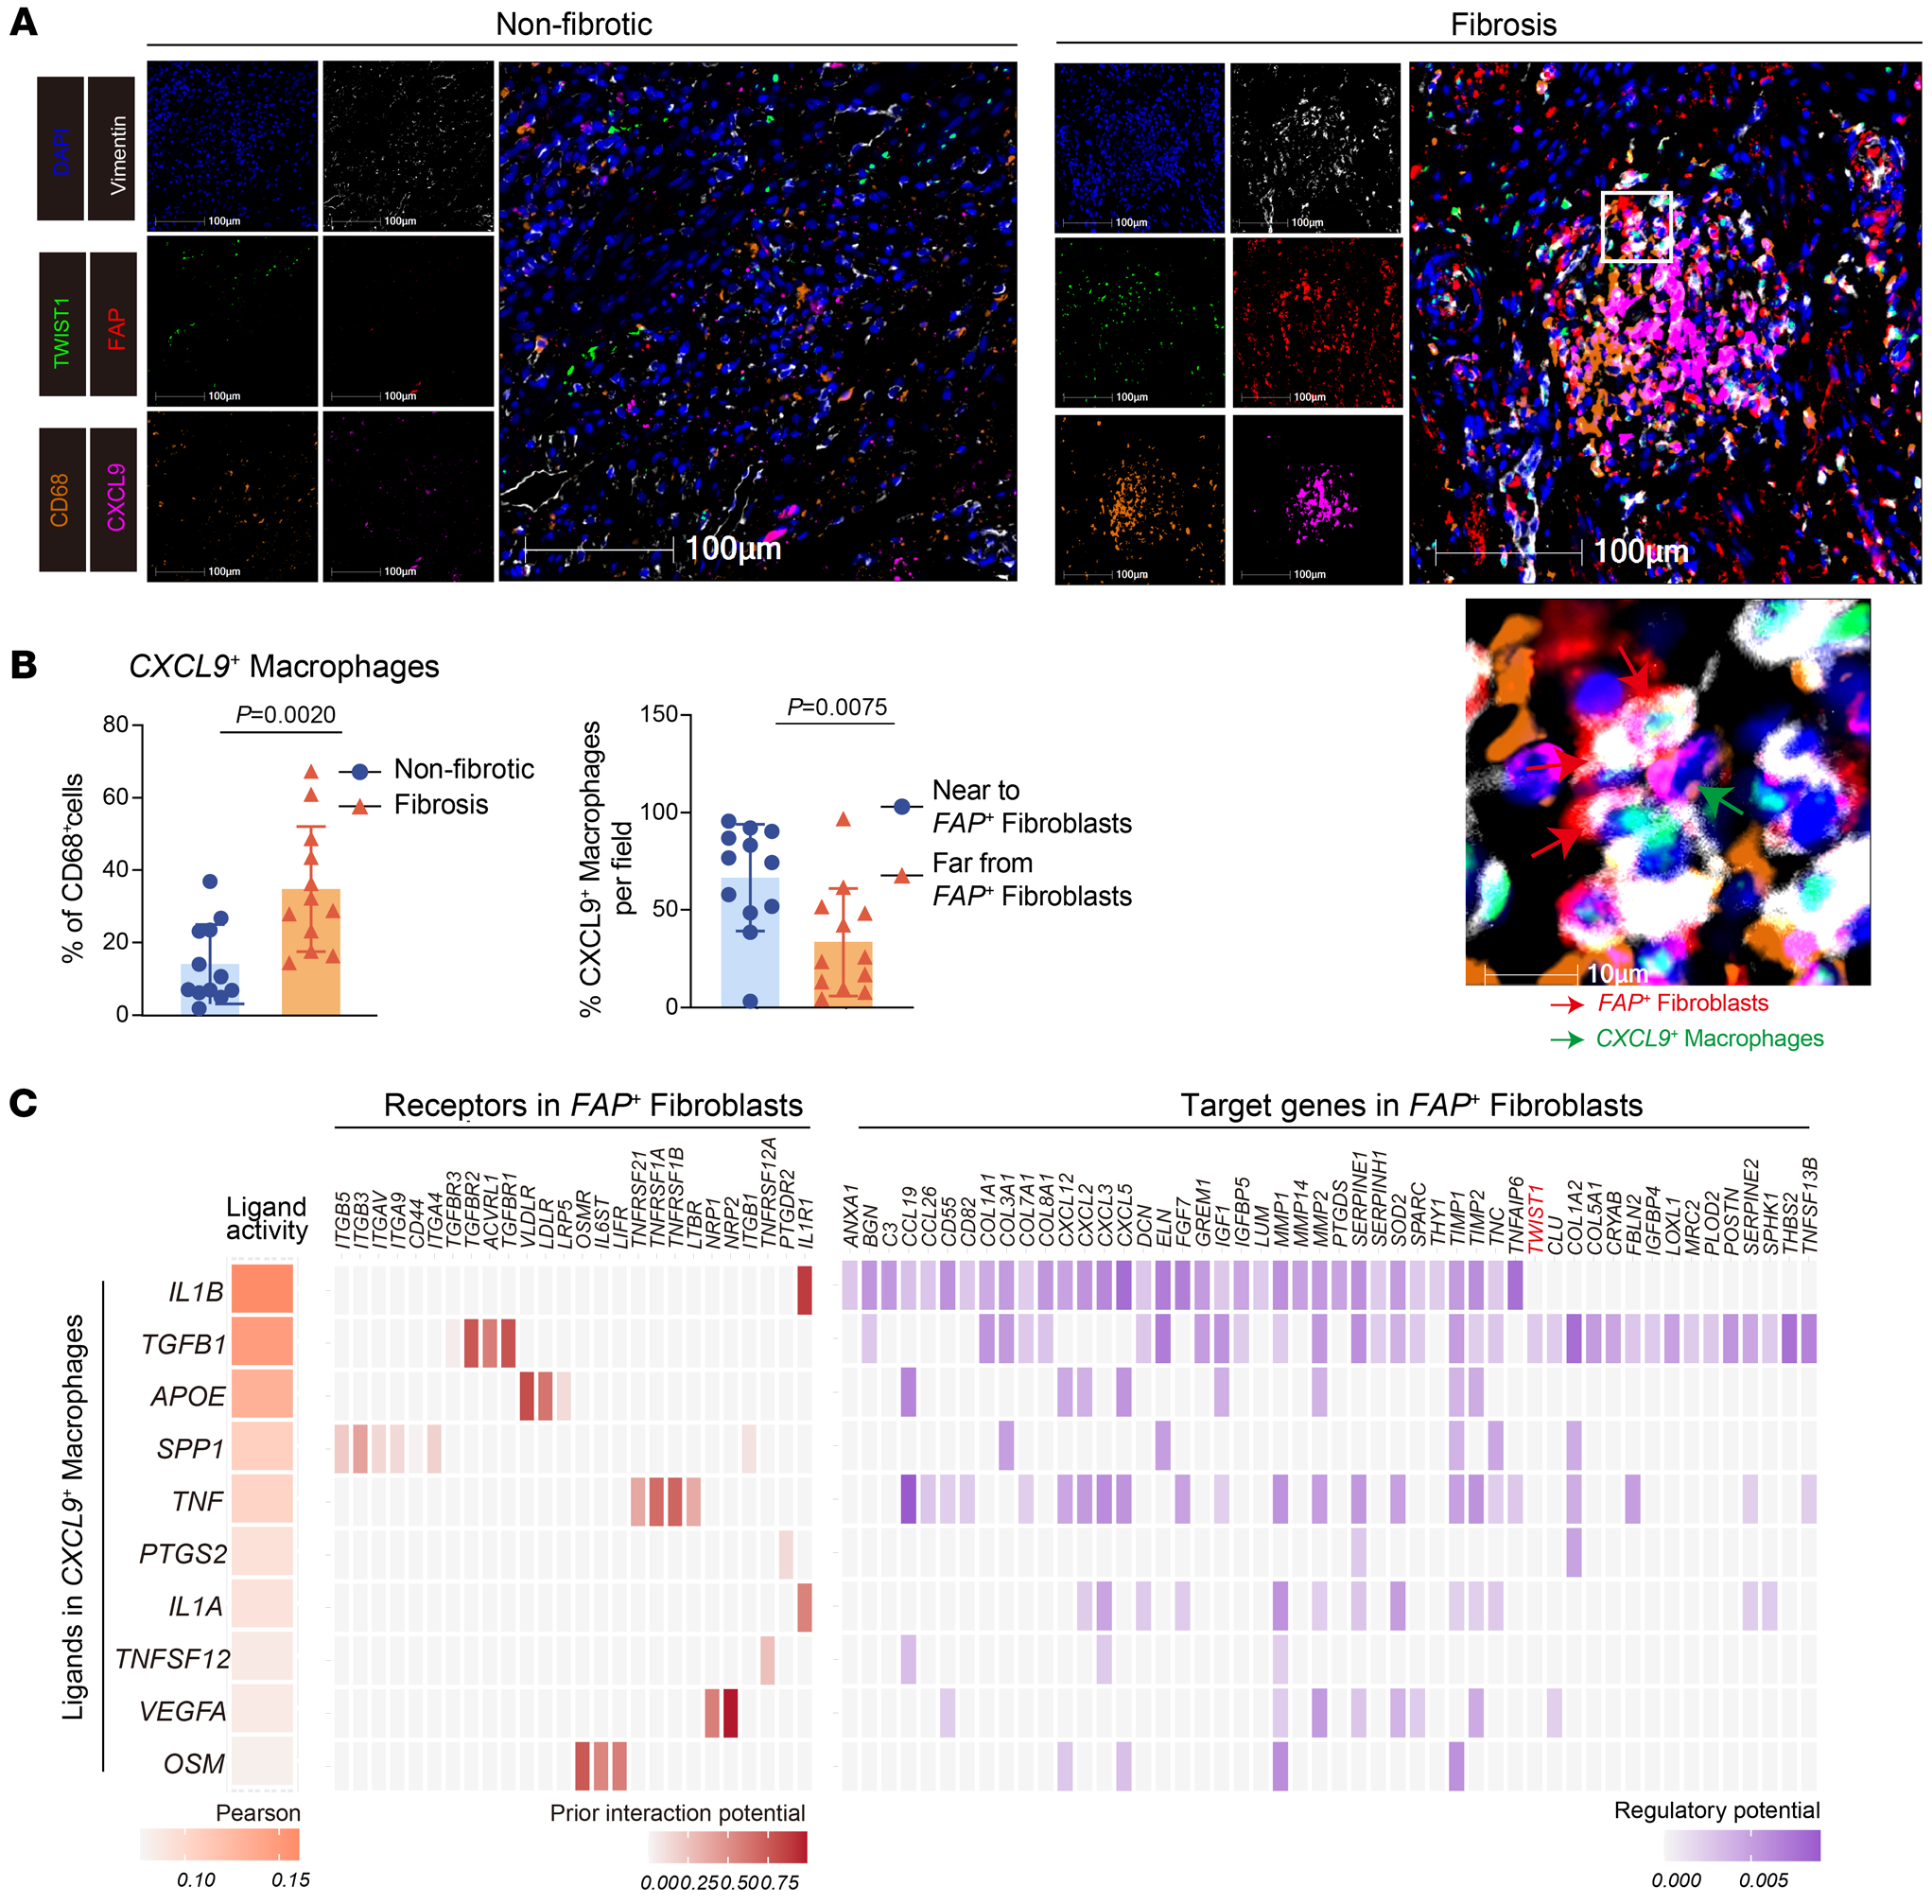
\includegraphics[width=\textwidth, trim=0 500 0 0, clip]{figures/fig5-img0.png}
{\tiny Source: Zhang et al., JCI 2024, Fig.\,5}

\column{0.47\textwidth}
\textbf{Multiplex IF (mIF)}:
\begin{itemize}
  \item CXCL9$^+$ Mac \HL{enriched} in fibrotic tissue
  \item \HL{Spatial proximity}: CXCL9$^+$ Mac adjacent to FAP$^+$ fibroblasts ($<$30\,$\mu$m)
\end{itemize}
\vspace{4pt}

\textbf{NicheNet analysis}:
\begin{itemize}
  \item CXCL9$^+$ Mac $\rightarrow$ high \textbf{IL1B} \& \textbf{TGFB1} ligand activity
  \item Receptors on FAP$^+$ Fib: IL1R1, TGFBR1/2, ACVRL1
  \item Downstream: collagen genes + \pos{TWIST1}
\end{itemize}
\vspace{4pt}

\begin{alertblock}{Mechanism}
CXCL9$^+$ Mac $\xrightarrow{\text{IL-1}\beta\text{/TGF-}\beta}$ \textbf{TWIST1} $\uparrow$ in FAP$^+$ Fib $\rightarrow$ ECM $\uparrow$
\end{alertblock}
\end{columns}
\end{frame}

% ============================================================
% SLIDE 10: Mouse Model — Cross-species Conservation (Fig 6)
% ============================================================
\begin{frame}{Cross-species Validation: DSS Mouse Fibrosis Model (Fig.\,6)}
\begin{columns}[T]
\column{0.52\textwidth}
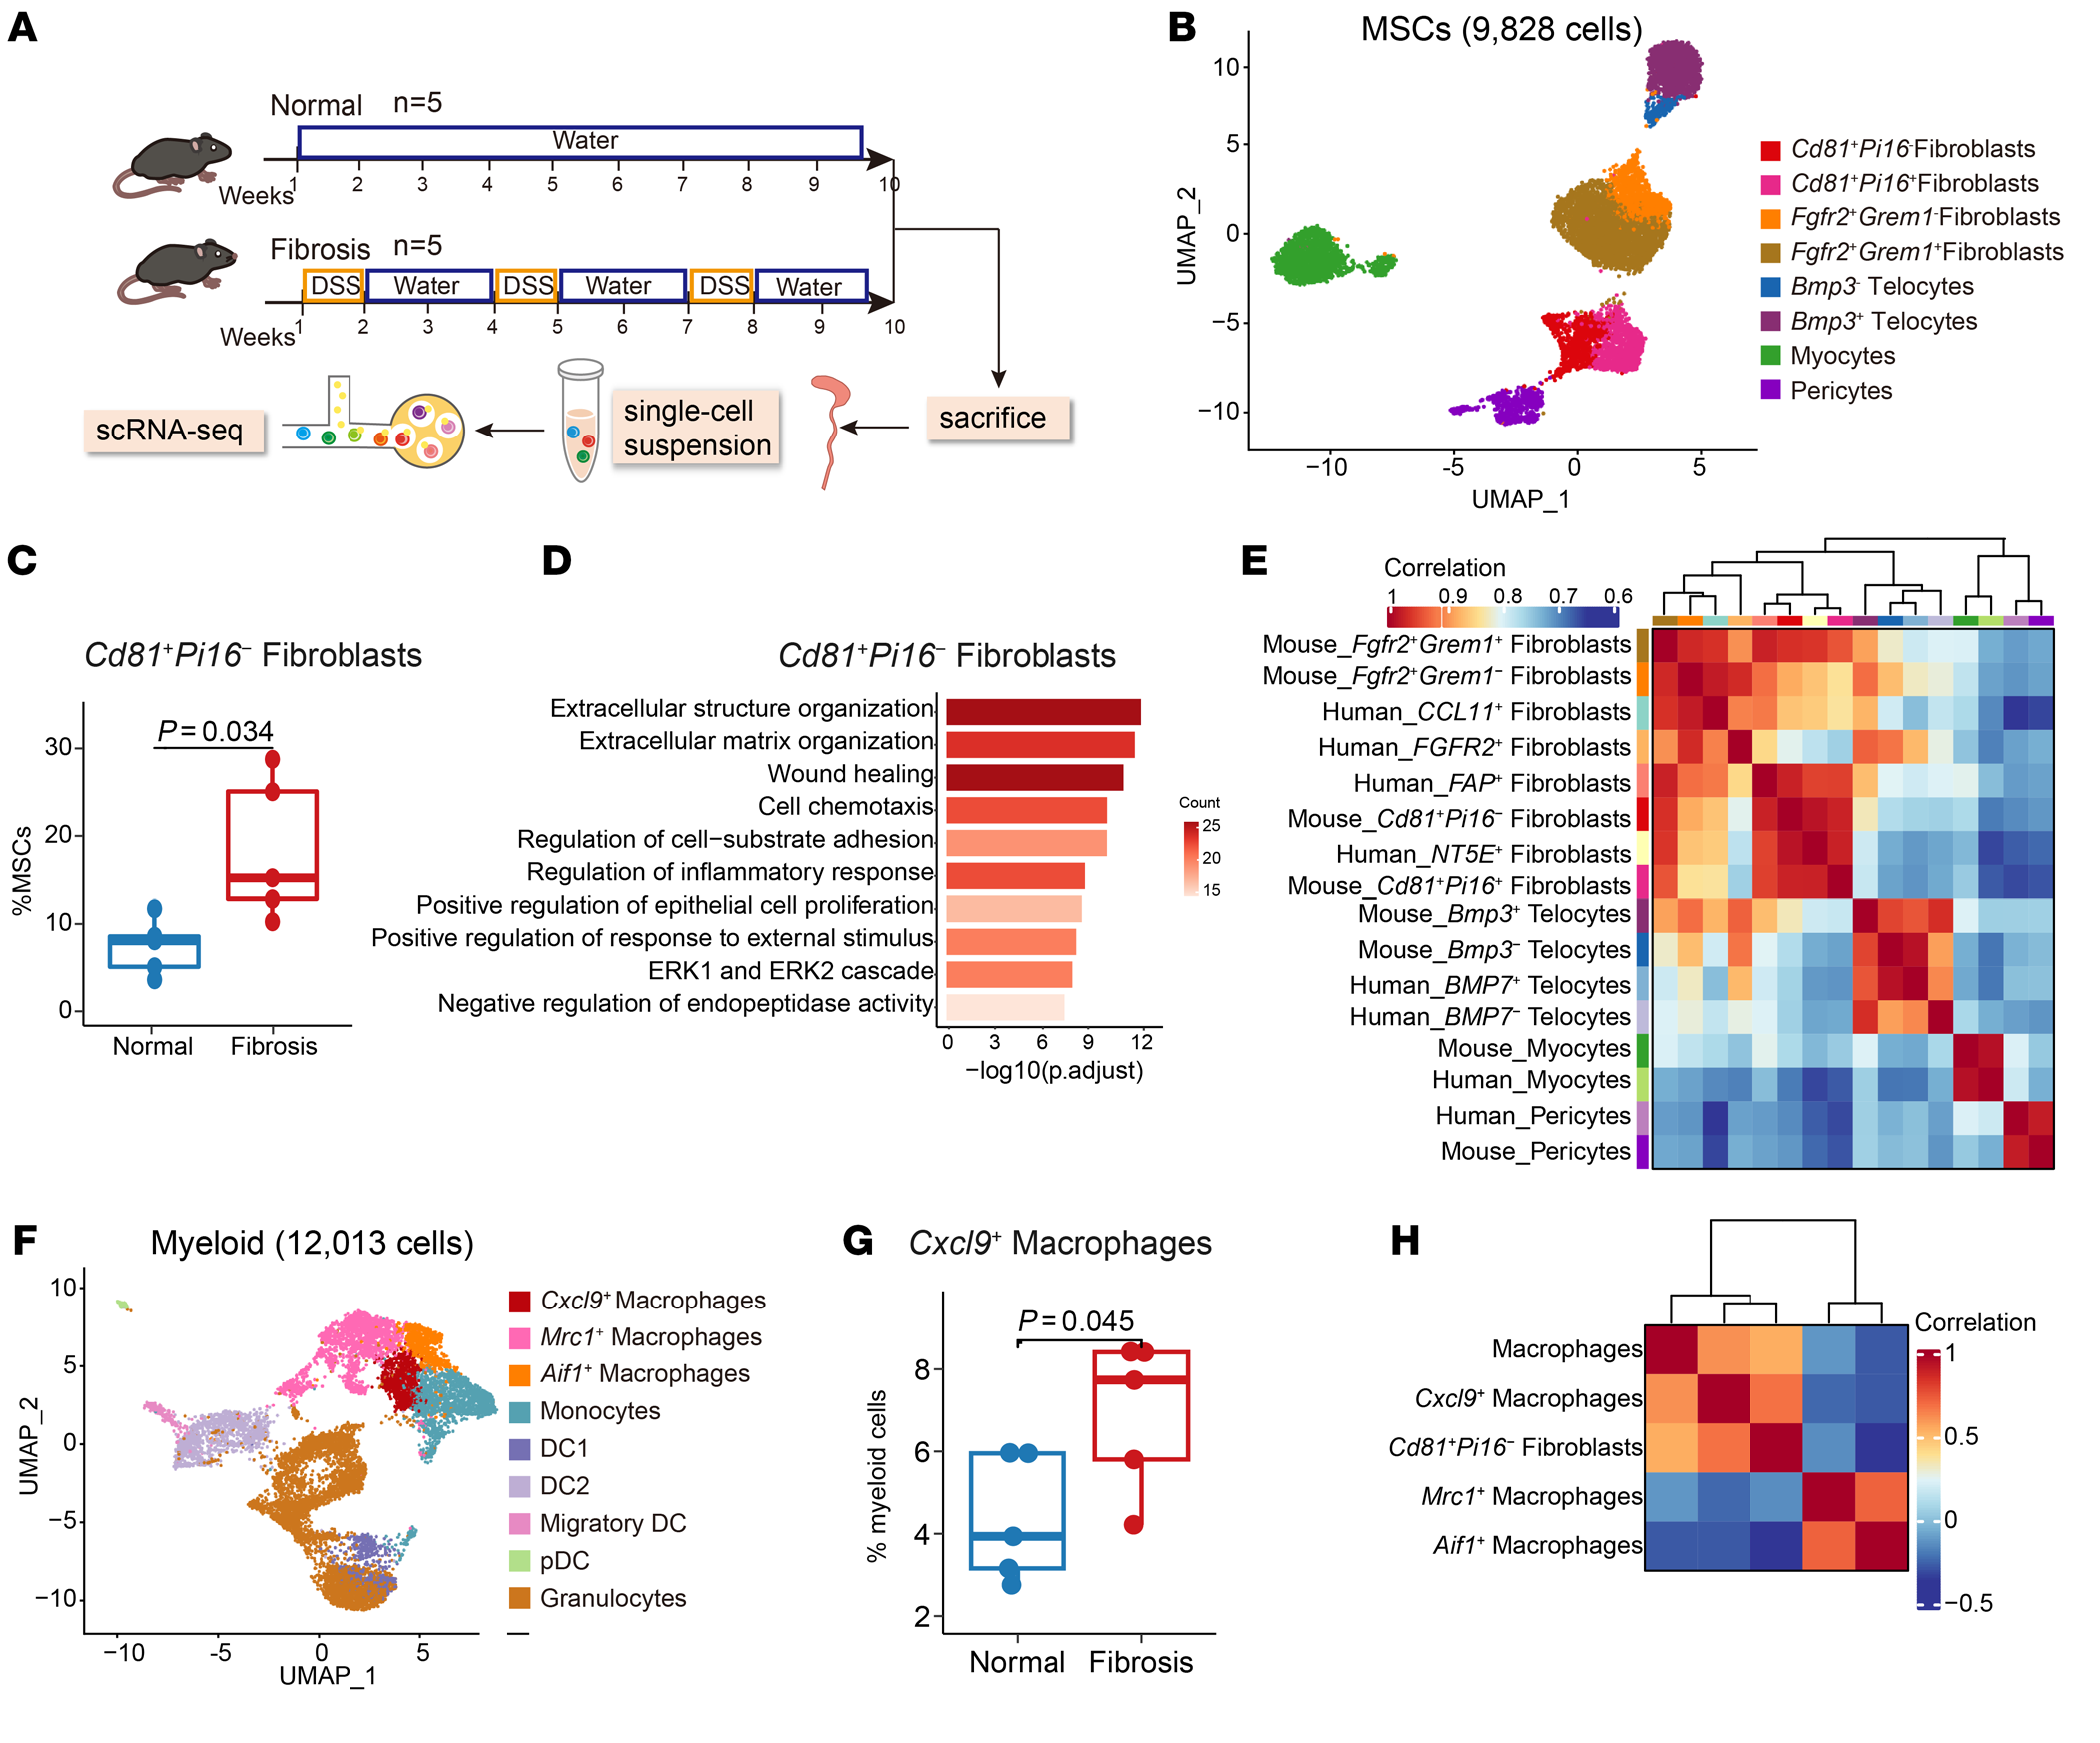
\includegraphics[width=\textwidth, trim=0 400 0 0, clip]{figures/fig6-img0.png}
{\tiny Source: Zhang et al., JCI 2024, Fig.\,6}

\column{0.45\textwidth}
\textbf{Chronic DSS model} $\rightarrow$ scRNA-seq:
\begin{itemize}
  \item 8 MSC subsets identified, including 4 fibroblast subtypes
\end{itemize}
\vspace{4pt}

\textbf{Mouse counterpart of FAP$^+$ Fib}:
\begin{itemize}
  \item \pos{CD81$^+$Pi16$^-$ fibroblasts}
  \item Enriched in fibrotic colon ($P = 0.034$)
  \item GO: ECM organization
  \item Transcriptomic \HL{cross-species conservation} with human FAP$^+$
\end{itemize}
\vspace{4pt}

\textbf{Mouse counterpart of CXCL9$^+$ Mac}:
\begin{itemize}
  \item \pos{Cxcl9$^+$ macrophages}
  \item Enriched in fibrosis ($P = 0.045$)
  \item Positive correlation with CD81$^+$Pi16$^-$ Fib
\end{itemize}
\end{columns}
\end{frame}

% ============================================================
% SLIDE 11: In Vitro — Harmine (Fig 7A)
% ============================================================
\begin{frame}{In Vitro: TWIST1 Inhibition Suppresses Fibroblast Activation (Fig.\,7A)}
\begin{columns}[T]
\column{0.50\textwidth}
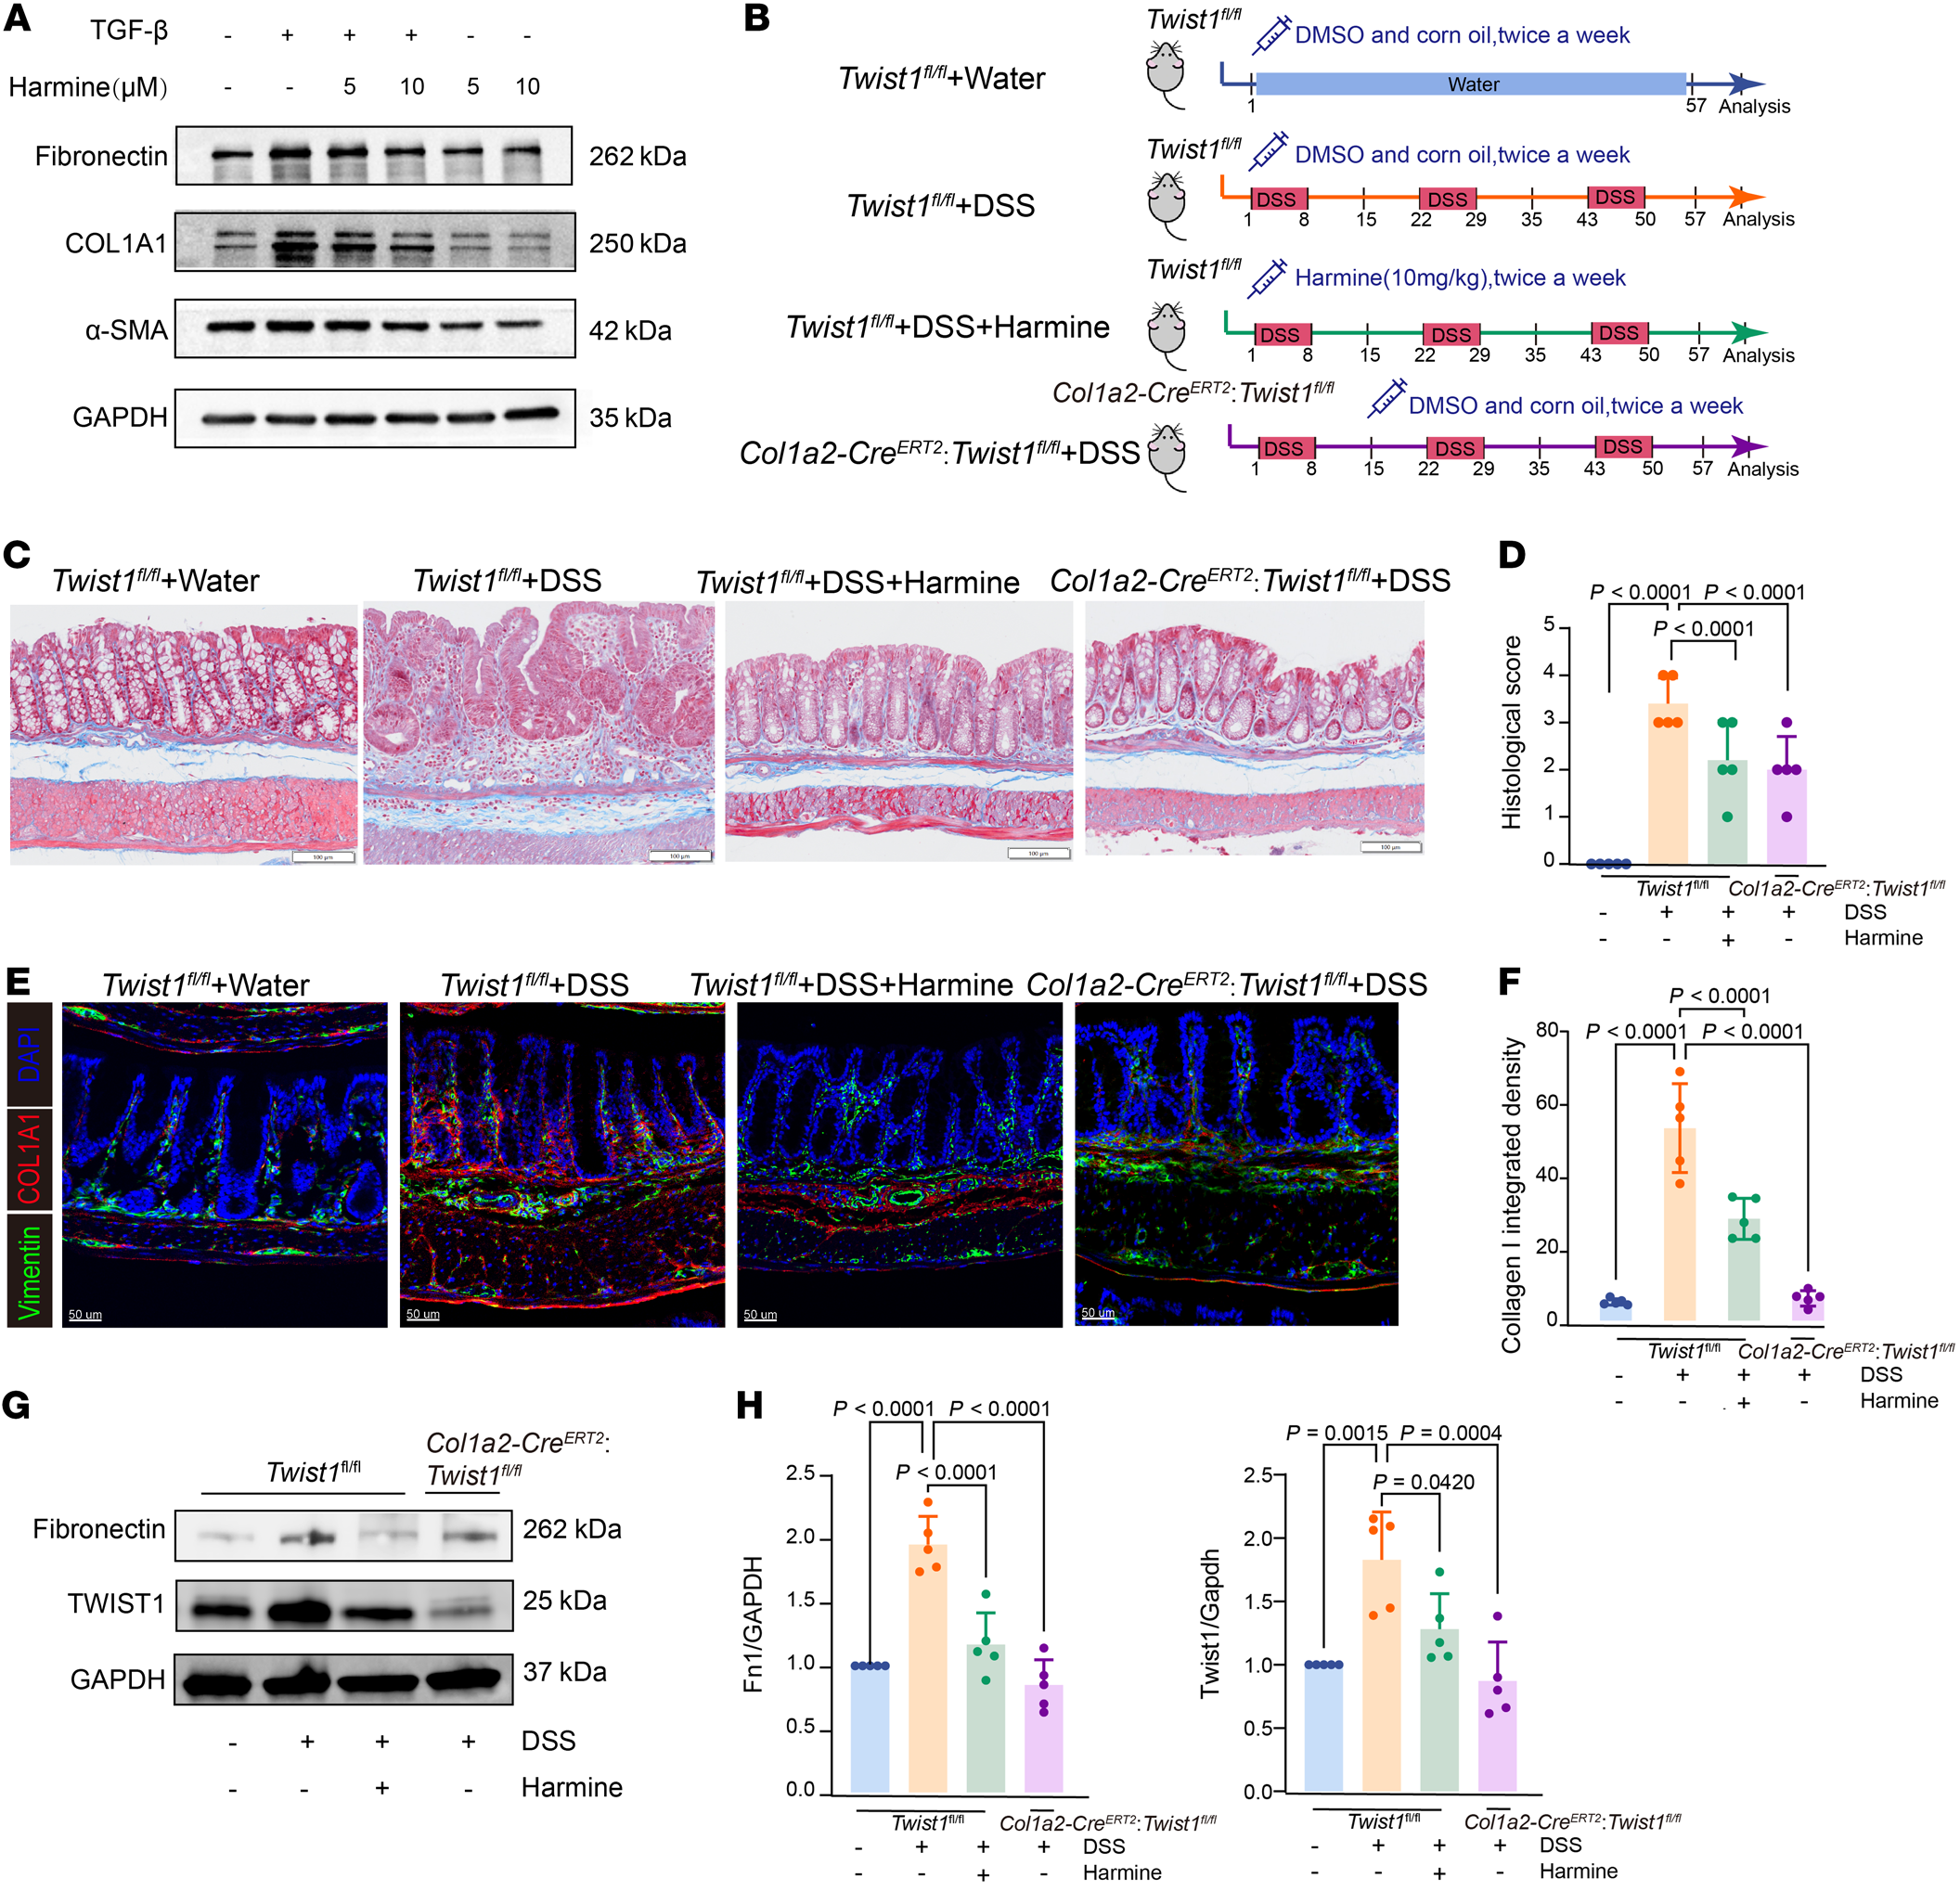
\includegraphics[width=\textwidth, trim=0 1050 900 0, clip]{figures/fig7-img0.png}
{\tiny Source: Zhang et al., JCI 2024, Fig.\,7A}

\column{0.47\textwidth}
\textbf{Experimental setup}:
\begin{itemize}
  \item Primary human intestinal fibroblasts
  \item TGF-$\beta$ stimulation (48h) $\rightarrow$ activation
  \item \textbf{Harmine}: TWIST1 inhibitor (induces degradation)
\end{itemize}
\vspace{4pt}

\textbf{Results}:
\begin{itemize}
  \item TGF-$\beta$ alone $\rightarrow$ \con{fibronectin $\uparrow$, $\alpha$-SMA $\uparrow$, COL1A1 $\uparrow$}
  \item TGF-$\beta$ + Harmine $\rightarrow$ \HL{markedly suppressed} all three markers
\end{itemize}
\vspace{4pt}

\begin{exampleblock}{Conclusion}
TWIST1 inhibition effectively suppresses fibroblast activation \& ECM production \textbf{in vitro}.
\end{exampleblock}
\end{columns}
\end{frame}

% ============================================================
% SLIDE 12: In Vivo — Twist1 KO & Harmine (Fig 7B-H)
% ============================================================
\begin{frame}{In Vivo: Targeting TWIST1 Attenuates Intestinal Fibrosis (Fig.\,7)}
\begin{columns}[T]
\column{0.50\textwidth}
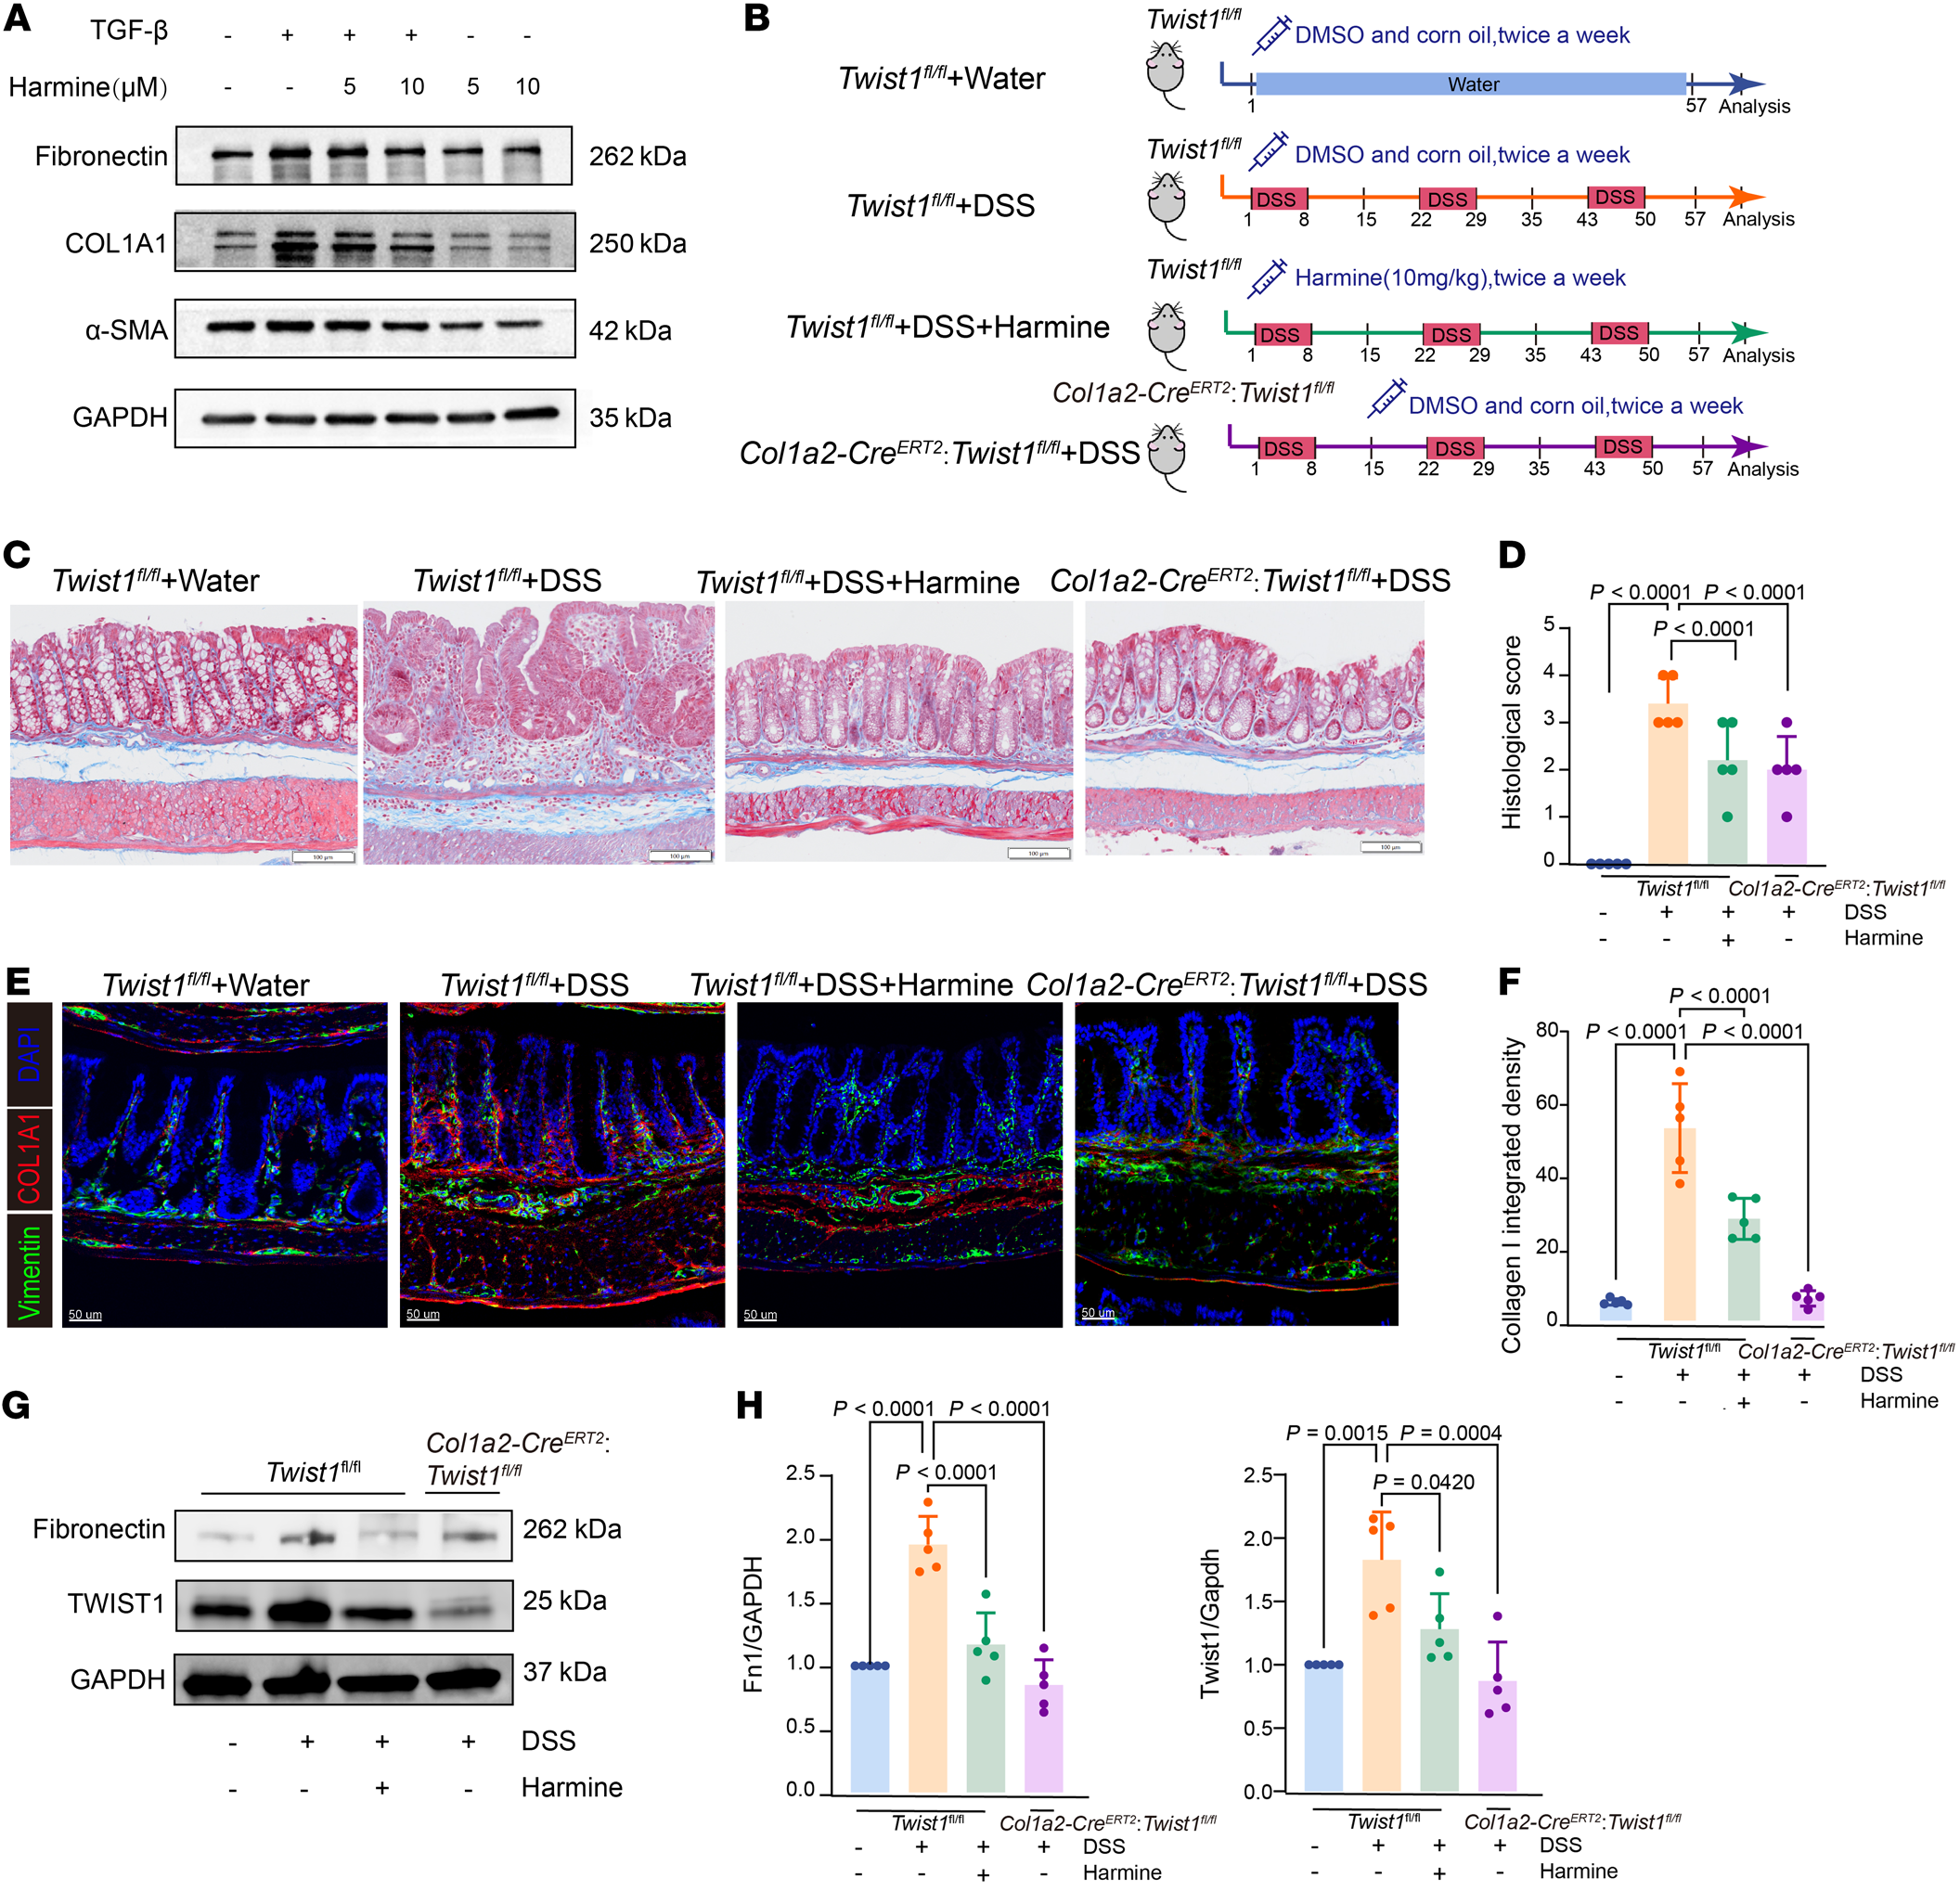
\includegraphics[width=\textwidth, trim=0 0 0 900, clip]{figures/fig7-img0.png}
{\tiny Source: Zhang et al., JCI 2024, Fig.\,7B--H}

\column{0.47\textwidth}
\textbf{Genetic approach}:
\begin{itemize}
  \item Col1a2-CreERT2 Twist1$^{fl/fl}$ mice
  \item Tamoxifen $\rightarrow$ fibroblast-specific Twist1 KO
  \item DSS-induced fibrosis model
\end{itemize}
\vspace{4pt}

\textbf{Both KO \& Harmine treatment}:
\begin{itemize}
  \item \HL{Reduced collagen deposition} (Masson's staining)
  \item \HL{Lower histological scores}
  \item \pos{Decreased} TWIST1, COL1A1 expression (IF)
  \item \pos{Decreased} ECM genes: TIMP-1, COL1A1, COL3A1, fibronectin
\end{itemize}
\vspace{4pt}

\textbf{Flow cytometry}: gp38$^+$CD81$^+$ MSCs \& CD206$^-$ Mac both \pos{reduced} after Twist1 KO under DSS.
\end{columns}
\end{frame}

% ============================================================
% SLIDE 13: Mechanistic Summary (TikZ Diagram)
% ============================================================
\begin{frame}{Proposed Mechanism}
\begin{center}
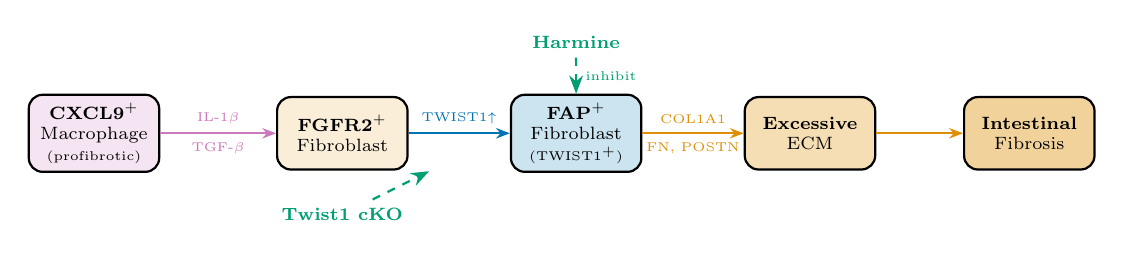
\begin{tikzpicture}[
  cell/.style={draw, rounded corners=5pt, minimum width=1.8cm, minimum height=1.0cm,
               font=\scriptsize, align=center, thick},
  signal/.style={-{Stealth[length=5pt]}, thick},
  node distance=0.8cm and 1.0cm,
  scale=0.92, every node/.append style={transform shape}
]
  % Macrophage
  \node[cell, fill=cbPurple!20] (mac) {\textbf{CXCL9$^+$}\\Macrophage\\{\tiny (profibrotic)}};

  % FGFR2+ fibroblast
  \node[cell, fill=negative!15, right=1.6cm of mac] (fgfr) {\textbf{FGFR2$^+$}\\Fibroblast};

  % FAP+ fibroblast
  \node[cell, fill=positive!20, right=1.4cm of fgfr] (fap) {\textbf{FAP$^+$}\\Fibroblast\\{\tiny (TWIST1$^+$)}};

  % ECM
  \node[cell, fill=negative!30, right=1.4cm of fap] (ecm) {\textbf{Excessive}\\ECM};

  % Fibrosis
  \node[cell, fill=negative!40, right=1.2cm of ecm] (fib) {\textbf{Intestinal}\\Fibrosis};

  % Arrows
  \draw[signal, cbPurple] (mac) -- node[above, font=\tiny] {IL-1$\beta$} node[below, font=\tiny] {TGF-$\beta$} (fgfr);
  \draw[signal, positive] (fgfr) -- node[above, font=\tiny] {TWIST1$\uparrow$} (fap);
  \draw[signal, negative] (fap) -- node[above, font=\tiny] {COL1A1} node[below, font=\tiny] {FN, POSTN} (ecm);
  \draw[signal, negative] (ecm) -- (fib);

  % Harmine inhibition
  \node[above=0.5cm of fap, font=\scriptsize] (harmine) {\HL{\textbf{Harmine}}};
  \draw[-{Stealth}, thick, emphasis, dashed] (harmine) -- node[right, font=\tiny] {inhibit} (fap);

  % KO
  \node[below=0.4cm of fgfr, font=\scriptsize] (ko) {\HL{\textbf{Twist1 cKO}}};
  \draw[-{Stealth}, thick, emphasis, dashed] (ko) -- ++(1.2,0.6);

\end{tikzpicture}
\end{center}
\vspace{-4pt}
\begin{itemize}
  \item CXCL9$^+$ macrophages secrete \textbf{IL-1$\beta$/TGF-$\beta$} $\rightarrow$ induce \textbf{TWIST1} in fibroblasts
  \item TWIST1 drives FGFR2$^+$ $\rightarrow$ FAP$^+$ fibroblast differentiation $\rightarrow$ excessive ECM
  \item \HL{Targeting TWIST1} (genetic KO or harmine) effectively \HL{attenuates fibrosis}
\end{itemize}
\end{frame}

% ============================================================
% SLIDE 14: Discussion & Significance
% ============================================================
\begin{frame}{Discussion \& Significance}
\begin{columns}[T]
\column{0.48\textwidth}
\begin{exampleblock}{Strengths}
\begin{itemize}
  \item First scRNA-seq on \textbf{surgical samples} (mucosa + submucosa) vs.\ endoscopic biopsy
  \item Identified \textbf{FAP$^+$ fibroblasts} as key ECM-producing cell type
  \item \textbf{Cross-species validation} (human $\leftrightarrow$ mouse)
  \item Both genetic \& pharmacological evidence for \textbf{TWIST1 as therapeutic target}
\end{itemize}
\end{exampleblock}

\column{0.48\textwidth}
\begin{alertblock}{Limitations \& Open Questions}
\begin{itemize}
  \item DSS model $\neq$ perfect recapitulation of human CD fibrosis
  \item Harmine has off-target effects (not specific to TWIST1)
  \item Epithelial cells underrepresented (enrichment for stromal \& hematopoietic)
  \item UC-related fibrosis: similar mechanism?
\end{itemize}
\end{alertblock}
\end{columns}
\vspace{6pt}

\textbf{Translational potential}:
$\quad$ TWIST1 inhibition $\rightarrow$ candidate antifibrotic strategy for CD strictures
\end{frame}

% ============================================================
% SLIDE 15: References
% ============================================================
\begin{frame}{References}
\begin{thebibliography}{9}
\small

\bibitem{zhang2024}
Zhang Y, Wang J, Sun H, et al.
TWIST1$^+$ FAP$^+$ fibroblasts in the pathogenesis of intestinal fibrosis in Crohn's disease.
\textit{J Clin Invest}. 2024;134(18):e179472.

\bibitem{rieder2017}
Rieder F, Fiocchi C, Rogler G.
Mechanisms, management, and treatment of fibrosis in patients with IBD.
\textit{Gastroenterology}. 2017;152(2):340--350.

\bibitem{kinchen2018}
Kinchen J, Chen HH, Parikh K, et al.
Structural remodeling of the human colonic mesenchyme in IBD.
\textit{Cell}. 2018;175(2):372--386.

\bibitem{davidson2020}
Davidson S, Coles M, Thomas T, et al.
Fibroblasts as immune regulators in infection, inflammation and cancer.
\textit{Nat Rev Immunol}. 2021;21(11):704--717.

\bibitem{smillie2019}
Smillie CS, Biton M, Ordovas-Montanes J, et al.
Intra- and inter-cellular rewiring of the human colon during UC.
\textit{Cell}. 2019;178(3):714--730.

\end{thebibliography}
\end{frame}

% ============================================================
% SLIDE 16: Thank You
% ============================================================
\begin{frame}[plain]
\vfill
\begin{center}
{\Large\bfseries Thank You}\\[12pt]
{\large Questions \& Discussion}\\[20pt]
{\small Presenter: [name]\\Shanghai Jiao Tong University\\[6pt]
Paper: Zhang et al., \textit{J Clin Invest}. 2024;134(18):e179472}
\end{center}
\vfill
\end{frame}

% ============================================================
% BACKUP SLIDES
% ============================================================
\appendix

\begin{frame}{Backup Slides}
\begin{center}
{\Large\bfseries Supplementary Materials}
\end{center}
\end{frame}

% BACKUP 1: Methods Detail
\begin{frame}{Methods: Sample Processing \& scRNA-seq}
\begin{columns}[T]
\column{0.48\textwidth}
\textbf{Sample collection}:
\begin{itemize}
  \item Fibrotic \& adjacent non-fibrotic ileal segments
  \item Patients with CD undergoing intestinal resection for fibrotic stricture
  \item Enriched for stromal \& hematopoietic cells
\end{itemize}
\vspace{4pt}
\textbf{Sequencing}:
\begin{itemize}
  \item 10x Genomics platform
  \item 91,316 cells post-QC (56,764 fibrotic + 34,552 non-fibrotic)
  \item Unsupervised clustering + marker gene annotation
\end{itemize}

\column{0.48\textwidth}
\textbf{Bioinformatics analyses}:
\begin{itemize}
  \item \textbf{SCENIC}: regulatory network inference for TF identification
  \item \textbf{RNA velocity} + \textbf{Monocle}: differentiation trajectory
  \item \textbf{NicheNet}: ligand--receptor interaction prediction
  \item ECM signature scoring (GO:0030198)
  \item Cross-species gene correlation (human vs.\ mouse)
\end{itemize}
\vspace{4pt}
\textbf{Mouse model}:
\begin{itemize}
  \item Chronic DSS-induced colitis/fibrosis
  \item Col1a2-CreERT2 Twist1$^{fl/fl}$ conditional KO
\end{itemize}
\end{columns}
\end{frame}

% BACKUP 2: Additional MSC Data
\begin{frame}{Supplementary: Additional MSC Subtype Analysis}
\textbf{Other MSC subsets \& their roles}:
\begin{center}
\begin{tabular}{llll}
\toprule
\textbf{Subset} & \textbf{Trend in Fibrosis} & \textbf{GO Enrichment} & \textbf{ECM Score} \\
\midrule
FAP$^+$ Fib & \pos{$\uparrow\uparrow$} & ECM organization & \textbf{Highest} \\
NT5E$^+$ Fib & $\uparrow$ & --- & Moderate \\
CCL11$^+$ Fib & --- & --- & Low \\
FGFR2$^+$ Fib & \con{$\downarrow$} & Inflammatory regulation & Low \\
Telocytes & --- & --- & Moderate \\
Pericytes & --- & Vascular regulation & Low \\
Myocytes & --- & Muscle contraction & Low \\
\bottomrule
\end{tabular}
\end{center}
\vspace{6pt}

\textbf{FAP expression in fibrosis}:
\begin{itemize}
  \item FAP mRNA and collagen-related genes both \pos{upregulated} in fibrotic areas
  \item COL1A1, ACTA2, POSTN significantly higher in FAP$^+$ Fib from fibrotic vs.\ non-fibrotic sites
\end{itemize}
\end{frame}

% BACKUP 3: Limitations & Future
\begin{frame}{Limitations \& Future Directions}
\begin{columns}[T]
\column{0.48\textwidth}
\textbf{Limitations}:
\begin{itemize}
  \item DSS model: chemically induced, not spontaneous CD-like fibrosis
  \item Harmine: DYRK1A kinase inhibitor with pleiotropic effects; not TWIST1-specific
  \item Epithelial/neuronal cells underrepresented due to enrichment protocol
  \item Small sample size (n=6 pairs)
  \item No longitudinal/temporal data on fibrosis progression
\end{itemize}

\column{0.48\textwidth}
\textbf{Future directions}:
\begin{itemize}
  \item Develop \textbf{TWIST1-specific inhibitors} or degraders
  \item Spatial transcriptomics for in situ validation
  \item Investigate UC-related fibrosis: same FAP$^+$ mechanism?
  \item Clinical trials: anti-TWIST1 therapy for CD strictures
  \item Single-cell multi-omics (ATAC-seq + RNA-seq) for epigenetic regulation
\end{itemize}
\end{columns}
\end{frame}

\end{document}
